\documentclass[11pt,oneside,a4paper]{book}
\usepackage[spanish]{babel}
\usepackage[latin1]{inputenc}
\usepackage[pdftex]{graphicx}           % para insertar figuras en formato pdf/png/jpg
\usepackage{color}
\usepackage{multirow}
\usepackage[table,xcdraw]{xcolor}
\usepackage{pifont}
\usepackage{amsfonts}
\usepackage{amssymb} 
\usepackage{setspace}
\usepackage[small,compact]{titlesec}
\usepackage{indentfirst} 
\usepackage[round]{natbib}
\usepackage{subfigure} 	
\usepackage[nottoc]{tocbibind}
\usepackage{setspace}
\usepackage{longtable}
\usepackage{lscape}
\usepackage{caption}
\usepackage{graphicx}
\usepackage{wrapfig}
\usepackage{lscape}
\usepackage{rotating}
\usepackage{epstopdf}
\usepackage{pdflscape}
\usepackage{amsmath}
\usepackage{listings}
\usepackage{color}
\usepackage{amsmath}
\usepackage{tcolorbox}
\usepackage{graphicx}
\usepackage{listings}
\usepackage{multirow}
\graphicspath{{../../02_figures/}}
\usepackage{longtable}
\usepackage{float}
\usepackage{adjustbox}
\usepackage[colorlinks=true,urlcolor=red,citecolor=green,linkcolor=blue]{hyperref}
\usepackage[a4paper,top=2.54cm, bottom=2.54cm, left=3cm, right=2.54cm]{geometry} %margenes
% ---------------------------------------------------------------------------- %
\graphicspath{{./figuras/}}
\makeindex  
\raggedbottom
\listfiles
\normalsize

\newcommand{\captionfonts}{\small}
\makeatletter  % Allow the use of @ in command names
\long\def\@makecaption#1#2{%
  \vskip\abovecaptionskip
  \sbox\@tempboxa{{\captionfonts #1: #2}}%
  \ifdim \wd\@tempboxa >\hsize
    {\captionfonts #1: #2\par}
  \else
    \hbox to\hsize{\hfil\box\@tempboxa\hfil}%
  \fi
  \vskip\belowcaptionskip}
\makeatother   % Cancel the effect of \makeatletter

\renewcommand{\topfraction}{0.85}
\renewcommand{\textfraction}{0.1}
\renewcommand{\floatpagefraction}{0.75}

% ---------------------------------------------------------------------------- %
% Cuerpo del texto
\begin{document}
\frontmatter \onehalfspacing

% ---------------------------------------------------------------------------- %
\thispagestyle{empty}
\begin{center}
\vspace*{1cm}
\textbf{\Large{PONTIFICIA UNIVERSIDAD CAT�LICA DEL PER� }}\\
\vspace*{1.2cm}

\textbf{\Large{ESCUELA DE GRADUADOS}}\\
\vspace*{0.5cm}
\begin{center}

\includegraphics[scale=.25]{logoPUCP}
\end{center}
\vspace{0.5cm}

\textbf{\Large{Modelo de regresi�n cuant�lica\\
  para respuestas positivas con censura intervalar}}\\
\vspace{1.2cm}
\textbf{\large{TESIS PARA OPTAR POR EL GRADO DE MAGISTER EN\\
  ESTAD�STICA}}\\
  
\vspace*{1.2cm}
\textbf{\large{Presentado por:}}\\
\vspace*{0.3cm}
\textbf{\large{Justo Andr�s Manrique Urbina}}\\
\vspace*{1.2cm}
\textbf{\large{Asesor: Cristian Luis Bayes Rodr�guez}}\\

\vspace*{1.2cm}

\textbf{\large{Miembros del jurado:\\
	Dr. Nombre completo jurado 1 \\
	Dr. Nombre completo jurado 2 \\
	Dr. Nombre completo jurado 3  
	}} 
	   
\vspace*{1.2cm}
    
\normalsize{Lima, Diciembre 2020}
\end{center}

% Agradecimentos
\chapter*{Agradecimientos}
A lo largo de la escritura de esta tesis de maestr�a he recibido un inmejorable soporte y asistencia. En primer lugar, quisiera agradecer a mi asesor, el profesor Cristian Bayes, cuya supervisi�n y consejos han sido invaluables para la elaboraci�n de este documento. La retroalimentaci�n recibida mejor� la calidad de las ideas expuestas aqu�. Asimismo, agradezco nuevamente al profesor Bayes y al profesor Giancarlo Sal y Rosas. Gracias a ambos, pude iniciar mi carrera acad�mica en Estad�stica. Finalmente, agradezco a la plana docente de la maestr�a por su ense�anza y orientaci�n durante los cursos llevados.


% ---------------------------------------------------------------------------- %
% Resumen
\chapter*{Resumen}

La presente tesis propone un modelo de regresi�n cuant�lica en d�nde la variable es no negativa y posee censura intervalar, es decir que esta no es directamente observable, y la �nica informaci�n que se conoce sobre ella es que se encuentra en cierto intervalo. Para evaluar si la metodolog�a de estimaci�n captura adecuadamente los par�metros poblacionales desde el punto de vista de la inferencia cl�sica, se desarrolla un estudio de simulaci�n. Finalmente, se aplica el modelo a los datos de la Encuesta Nacional de Satisfacci�n de Salud ejecutada el a�o 2015. La estructura del modelo permite evaluar los factores relacionados al sueldo de los profesionales en salud (el cual hab�a sido censurado desde el proceso de recolecci�n de datos). El presente modelo es una extensi�n al modelo de regresi�n de censura intervalar expuesto en \cite{salyrosas:bayes}, pues eval�a los factores subyacentes a una variable respuesta a lo largo de sus cuantiles.

\noindent \textbf{Palabras clave:} censura intervalar, regresi�n con censura, inferencia cl�sica, regresi�n param�trica.

% ---------------------------------------------------------------------------- %
% Indice
\tableofcontents    % imprime el indice
% ---------------------------------------------------------------------------- %


\chapter{Lista de S�mbolos}
\begin{tabular}{ll}
	$Y \sim W_r(q_{t},\alpha)$	& Variable $Y$ sigue una distribuci�n Weibull reparametrizada. \\
	$q_t$				& Par�metro de forma. \\
	$\alpha$    			& Par�metro de escala.\\

\end{tabular}

\listoffigures               % lista de Figuras
\listoftables                % lista de cuadros

% ---------------------------------------------------------------------------- %
\mainmatter

\onehalfspacing              % interlineado 1.5

%% ------------------------------------------------------------------------- %%
\chapter{Introducci�n}
\label{cap:introduccion}

%% ------------------------------------------------------------------------- %%
Por distintas razones, los datos recabados en una investigaci�n de �ndole estad�stica carecen de precisi�n: existen discrepancias entre el valor real del objeto de medici�n y el valor obtenido. Este proceso puede ser sist�mico: durante la administraci�n de cuestionarios a una poblaci�n objetivo, el encuestado puede omitir, reh�sar o incluso responder incorrectamente preguntas embarazosas o invasivas. Este dilema es conocido entre los encuestadores: sus encuestados, si bien est�n dispuestos a ofrecer la mejor ayuda posible, no est�n dispuestos a ofrecer informaci�n que posteriormente les pueda comprometer. Para obtener dichos datos, el encuestador usa todo su ingenio para equilibrar la privacidad del encuestado y los objetivos de su investigaci�n. En un esfuerzo de aminorar el estr�s del encuestado, el encuestador puede censurar los datos con el fin de obtener una respuesta.

Dichos datos censurados han sido estudiados previamente en la literatura acad�mica. Formalmente, y siguiendo las ideas plasmadas por \cite{peto:p}, una variable $C$ se le denota censurada cuando su valor $c$ no es del todo observable y la �nica informaci�n sobre la misma es un intervalo no-cero $I$. Esta construcci�n permite definir tres tipos de datos censurados: datos censurados \textit{hacia la izquierda} (en d�nde el intervalo $I$ se define de la forma $[-\infty,L_i]$), datos censurados \textit{intervalares} (definido de la forma $[L_i, L_f]; L_i < L_f$), datos censurados \textit{hacia la derecha} (definido de la forma $[L_f, \infty]$). Este tipo de datos naturalmente generan retos en el proceso de modelamiento, pues los modelos est�ndares de regresi�n presumen que la variable respuesta es directamente observable.

Situaciones como la precisada en el parr�fo precedente han sido exploradas previamente: desde la determinaci�n de la verosimilitud, la elaboraci�n de modelos de regresi�n y su estimaci�n bajo inferencia cl�sica y bayesiana. \cite{gentleman:lmk} identificaron un m�todo de m�xima verosimilitud para este tipo de datos, asegurando su consistencia estad�stica e identificando m�todos algor�tmicos para su c�mputo. Utilizado los puntos extremos del intervalo, $L_i$ y $L_f$, era posible identificar la m�xima veros�militud a trav�s de la diferencia de las funciones de distribuci�n acumulada en dichos puntos. Tomando en consideraci�n dicho m�todo de estimaci�n, distintos autores propusieron modelos de regresi�n param�tricos bajo inferencia cl�sica y bayesiana, tales como \cite{mun:xu}, quienes identificaron modelos param�tricos de supervivencia para este tipo de datos.

Cabe resaltar que los modelos anteriormente expuestos identifican el valor esperado de la variable respuesta condicionada por un conjunto de variables. Sin embargo, el inter�s del investigador puede recaer en otro objetivo: m�s all� de la respuesta media, el investigador busca los factores subyacentes que impactan a distintos cuantiles de la variable respuesta. Los factores relacionados a una persona con un gran sueldo son distintos a una persona que no percibe mucho. Para estudios de dicho corte, los modelos de regresi�n cuant�lica brinda la flexibilidad requerida. Dicho modelo fue propuesto inicialmente por Koenker y Basset (1978) quienes, ante la situaci�n en d�nde la estimaci�n de m�nimos cuadrados es deficiente en modelos con errores no gaussianos, proponen una regresi�n de cuantiles que permiten modelar libremente los cuantiles de la variable respuesta en relaci�n a las covariables.

\textbf{Pendiente: Texto explicando los estudios de regresi�n cuant�lica con censura intervalar}

La presente tesis propone utilizar los temas y modelos anteriormente expuestos para implementar un modelo param�trico de regresi�n cuant�lica aplicado a datos con censura intervalar. Para efectos de la aplicaci�n, los datos se modelar�n bajo una distribuci�n Weibull, la cual es de amplia aplicabilidad y permite modelar colas pesadas. Con el prop�sito de implementar la regresi�n cuant�lica y, atendiendo a la estructura de los datos, dicha distribuci�n ser� reparametrizada. Finalmente, el m�todo de estimaci�n ser� el de m�xima verosimilitud, siguiendo el marco de la inferencia cl�sica.

\section{Objetivos}
\label{sec:objetivo}

El objetivo de la tesis consiste en proponer un m�todo de regresi�n cu�ntiliza adaptado a datos con censura intervalar. Para identificar que el modelo propuesto es adecuado, aplicaremos la regresi�n en dos conjuntos de datos: uno simulado y otro real. La base de datos a utilizar ser� la Encuesta Nacional de Satisfacci�n de Usuarios en Salud elaborada por el Instituto Nacional de Estad�stica e Inform�tica el a�o 2015. Los objetivos espec�ficos de la tesis son los siguientes:

\begin{itemize}
	\item Revisar literatura acad�mica relacionada a las propuestas de modelos de regresi�n con datos censurados intervalarmente.
	\item Identificar una estructura apropiada de la distribuci�n Weibull para el modelo de regresi�n cuant�lica v�a una reparametrizaci�n del modelo. Posteriormente, estudiar el comportamiento de dicha estructura.
	\item Estimar los par�metros del modelo propuesto bajo inferencia cl�sica.
	\item Implementar el m�todo de estimaci�n para el modelo propuesto en el lenguaje R y aplicarlo en datos simulados.
	\item Aplicar el modelo propuesto en datos de la Encuesta Nacional de Satisfacci�n de Usuarios en Salud.
\end{itemize}

\section{Organizaci�n del Trabajo}
\label{sec:organizacion}

En el cap�tulo 2, se presenta una estructura de la distribuci�n Weibull, apropiada para los datos con censura intervalar. Por ello, se realiza una parametrizaci�n alternativa y se estudia los 

En el cap�tulo 3, se propone el modelo de regresi�n con datos censurados intervalarmente.

En el cap�tulo 4, se presenta la aplicaci�n del modelo propuesto para determinar si existe diferencia entre los sueldos de enfermeras y enfermeros a lo largo de todos los cuantiles. Ello se realiza mediante inferencia cl�sica.

Finalmente, en el cap�tulo 5 se presentan las principales conclusiones obtenidas en la presente tesis as� como los pr�ximos pasos.

\chapter{Distribuci�n de Weibull}

El presente cap�tulo tiene como objetivo principal proponer una reparametrizaci�n de la distribuci�n de Weibull para adaptarla al modelo de regresi�n cuant�lica. Para dicha reparametrizaci�n, se definir� su funci�n de densidad y funci�n de distribuci�n acumulada, y asimismo se examinar� sus propiedades.

\section{Distribuci�n de Weibull}

La distribuci�n de Weibull fue introducida por \cite{weib:weib}. En dicho art�culo de investigaci�n, Weibull menciona las caracter�sticas de una funci�n de densidad suficientemente flexible para ser adaptada a diversas investigaciones, desde la rama de resistencia de materiales hasta el an�lisis de altura de hombres adultos radicados en las Islas Brit�nicas. Una variable aleatoria continua $Y$, con soporte $Y \in (0,\infty)$, sigue una distribuci�n de Weibull si su funci�n de densidad es dada por la siguiente expresi�n:

\begin{equation}
f{(y)}= \frac{\alpha}{\sigma}\left(\frac{y}{\sigma}\right)^{\alpha-1} \exp{\left(-\frac{y}{\sigma}\right)^{\alpha}}
\end{equation}

\noindent en donde $\alpha > 0$ corresponde al par�metro de forma, y $\sigma > 0$ corresponde al par�metro de escala. La notaci�n de una variable aleatoria $Y$ que sigue esta distribuci�n se indica como $Y \sim W(\alpha,\sigma)$. La funci�n de distribuci�n acumulada de $Y$ tiene la siguiente expresi�n:

\[F{(y)}=1-\exp^{-{(\frac{y}{\sigma})}^{\alpha}}.\]

\noindent Asimismo, su funci�n de cuantiles es dada por:

\[q_{t}=\sigma{(-\log{(1-t)})}^{\frac{1}{\alpha}}\]

\noindent para $0 < t < 1$.

La flexibilidad referida por la distribuci�n de Weibull puede observarse a trav�s de la figura \ref{weib:original}. En dicha figura, observamos que una modificaci�n del par�metro de escala $\sigma$ modifica la tendencia central de la distribuci�n; es decir, se observa que la distribuci�n se mueve en la direcci�n que el par�metro $\sigma$ se mueve. Cabe resaltar que, con un $\alpha$ fijo, la distribuci�n tiende a ser m�s dispersa. Por otro lado, se observa que el aumento del par�metro de forma $\alpha$ contrae la distribuci�n hacia el valor central de la misma. Esto es m�s pronunciado en la medida que dicho par�metro aumenta, manteniendo el par�metro $\sigma$ constante. No obstante, cabe resaltar que la distribuci�n se torna asim�trica en tanto los valores de $\alpha$ son peque�os.

\begin{figure}
	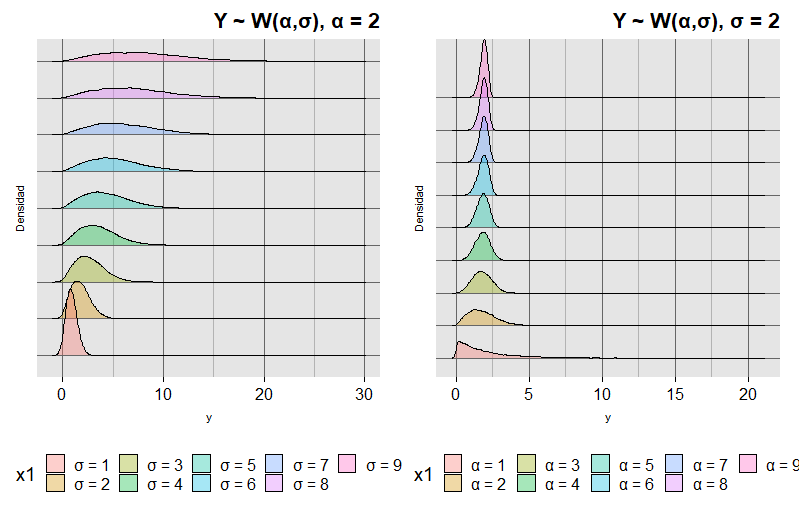
\includegraphics[width=\textwidth]{weib_distrib}
	\caption{Funci�n de densidad de una variable $Y$ con distribuci�n Weibull}
	\label{weib:original}
\end{figure}

Para una variable $Y \sim W(\alpha, \sigma)$, la media y varianza se definen de la siguiente forma:

\[E(Y)=\sigma \Gamma\left( 1+\frac{1}{\alpha} \right).\]
\[V(Y)=\sigma^{2}\left[ \Gamma\left( 1+\frac{2}{\alpha} \right)-\left( \Gamma\left( 1+\frac{1}{\alpha} \right) \right)^{2} \right].\]

\noindent donde $\Gamma(\cdot)$ es la funci�n Gamma.
\section{Hacia una nueva estructura de la distribuci�n de Weibull}
\label{sec2.2}

En esta secci�n consideramos una reparametrizaci�n del par�metro de forma $\sigma$ en t�rminos del cuantil $t, q_{t}$ en los siguientes t�rminos:

\[\sigma = \frac{q_t}{(-\log(1-t))^{\frac{1}{\alpha}}} \]

\noindent en donde $t$ ser� un valor conocido que se encuentra en el intervalo $[0,1]$. Bajo esta nueva estructura, $q_{t}$ y $\alpha$ tienen espacios param�tricos independientes tal que $(q_{t},\alpha) \in (0,\infty) \times (0,\infty)$. Una variable aleatoria $Y$ que sigue una distribuci�n Weibull bajo esta parametrizaci�n se denota como $Y \sim W_{r}(q_{t},\alpha,t)$ y posee la siguiente funci�n de densidad:

\begin{equation}
f_{Y}(y| q_{t},\alpha,t)=\frac{\alpha c(t)}{q_{t}}\left( \frac{y}{q_{t}} \right)^{\alpha-1}\exp\left( -c(t)\left( \frac{y}{q_{t}} \right)^{\alpha} \right)
\end{equation}
\\
\noindent donde $c(t)= \left( -\log(1-t) \right)$. 

Los par�metros $q_{t}$ y $\alpha$, as� como el nivel del cuantil $t$ (el cual es conocido), caracterizan la funci�n de densidad conforme se observa en la Figura \ref{fig:newdens}. En dicha figura, se observa el efecto del nuevo par�metro $q_t$ y el nivel $t$. Podemos observar lo siguiente: 

\begin{itemize}
	\item Se observa que una variaci�n del par�metro $q_t$ conlleva a un aumento en la tendencia central de la distribuci�n hacia la misma direcci�n (en la medida que el par�metro de escala $\alpha$ es constante). Asimismo, para valores bajos de $q_t$, la distribuci�n es leptoc�rtica concolas pronunciadas a la derecha. Asimismo, dicho aumento del par�metro genera valores extremos: la distribuci�n se torna asim�trica, con valores extremos generados cada vez con mayor frecuencia.
	\item Se observa que, para un mismo par�metro $q_t$, la distribuci�n es platic�rtica en la medida que se observe los cuantiles inferiores. Asimismo, en determinados casos pronuncia la asimetr�a identificada anteriormente.
\end{itemize}

\begin{landscape}
\begin{figure}
\centering
	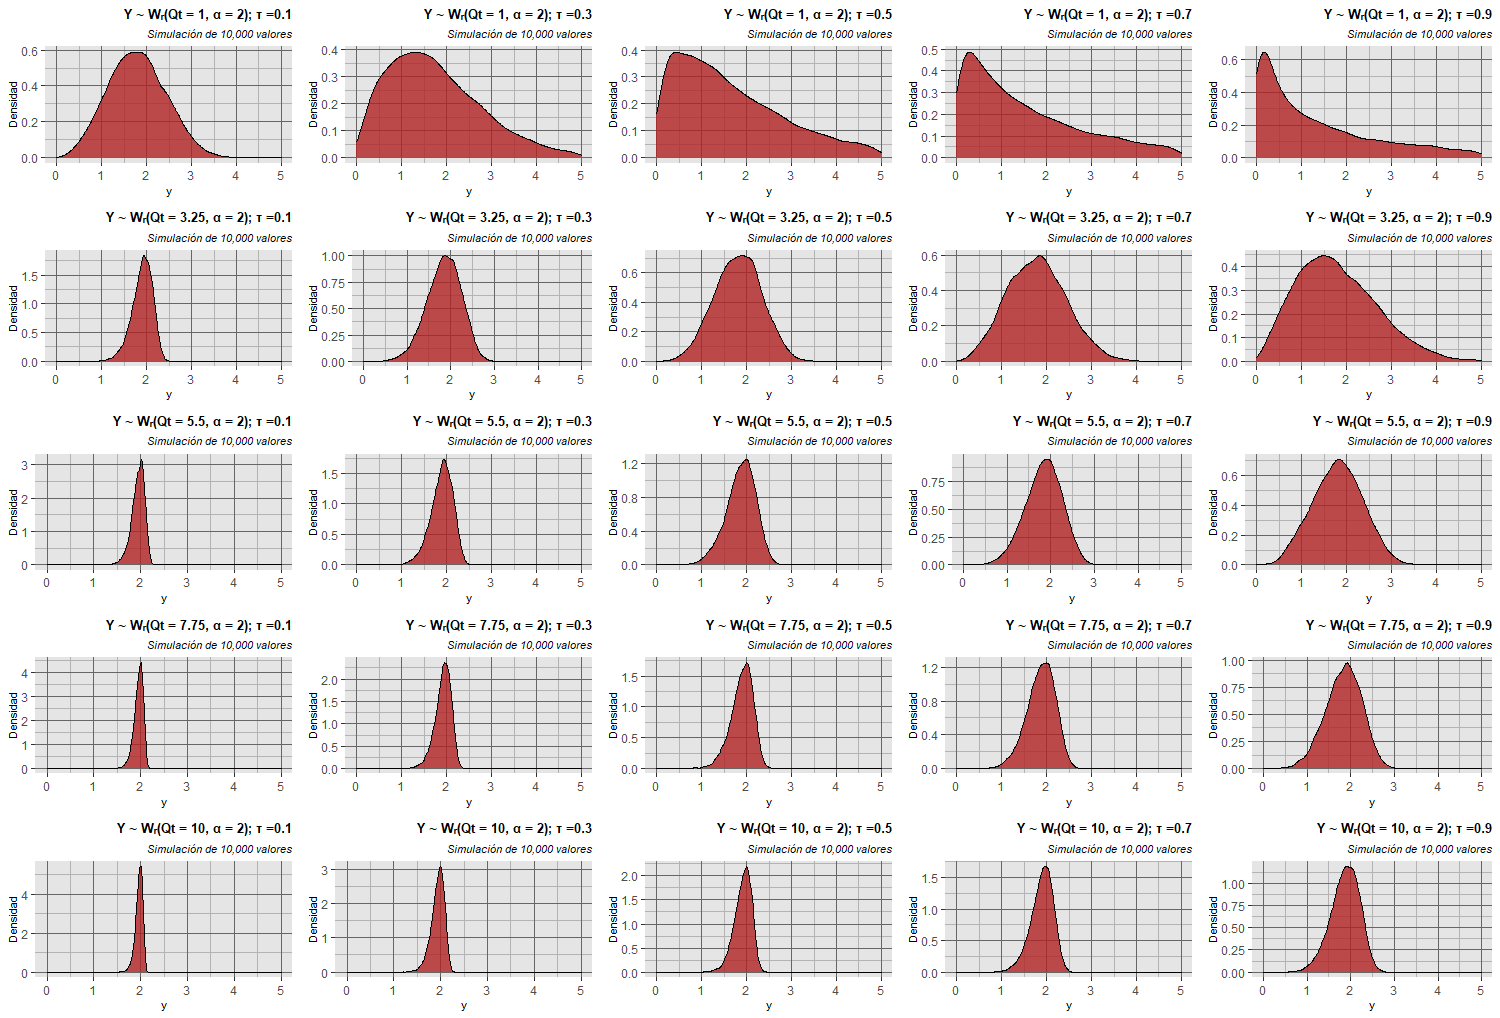
\includegraphics[width=1.5\textheight]{rep_weibull_qt}
	\caption{Densidades de la distribuci�n de Weibull bajo la nueva parametrizaci�n}
	\label{fig:newdens}
\end{figure}
\end{landscape}

\begin{landscape}
	\begin{figure}
		\centering
		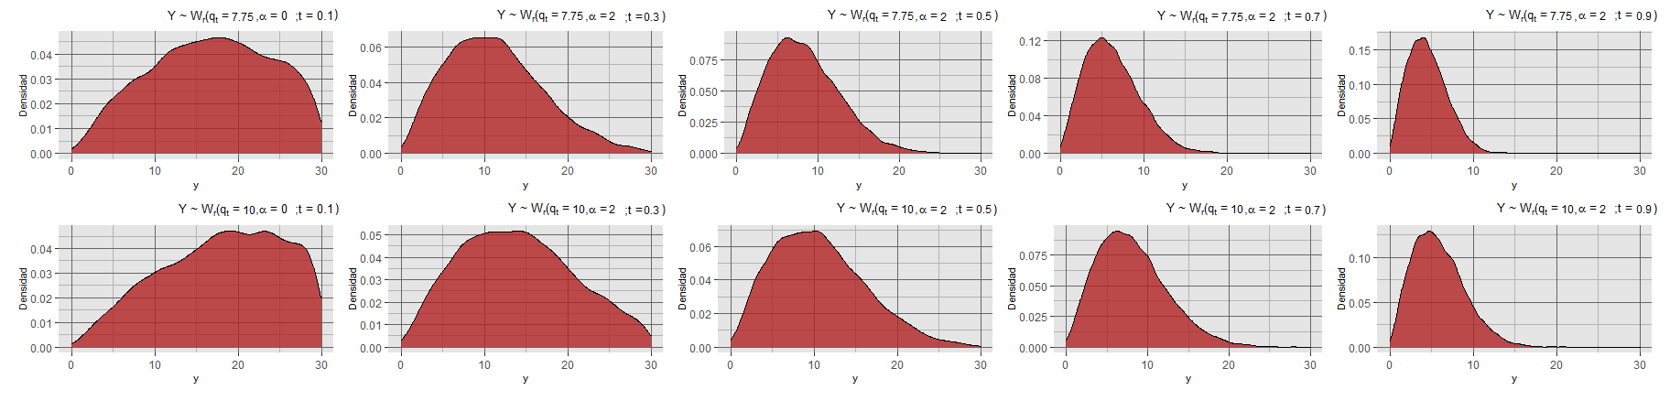
\includegraphics[width=1.5\textheight]{rep_weibull_qt_2}
		\caption{Densidades de la distribuci�n de Weibull bajo la nueva parametrizaci�n}
		\label{fig:newdens2}
	\end{figure}
\end{landscape}

En base a la reparametrizaci�n propuesta, la funci�n de distribuci�n acumulada de $Y \sim W_r(q_t,\alpha,t)$ es de la forma:

\begin{equation} \label{eq:1}
	F_{Y}\left(y| q_{t},\alpha,t \right)=1-\exp\left( -log(1-t)\left( \frac{y}{q_{t}} \right)^{\alpha} \right).
\end{equation}

\noindent Recordemos que $e^{a log(z)} = z^a$, en d�nde $a = -\left(\frac{y}{q_{t}} \right)^{\alpha}$ y $z = (1-t)$. Por lo tanto tenemos:

\begin{equation} \label{eq:2}
F_{Y}\left(y| q_{t},\alpha,t \right)=1-(1-t)^{-\left(\frac{y}{q_{t}} \right)^{\alpha}}.
\end{equation}


Asimismo, el valor esperado y varianza de dicha variable aleatoria est� dada por:

\begin{equation}
E(Y)=\frac{q_{t}}{c(t)^{\frac{1}{\alpha}}}\Gamma\left( 1+\frac{1}{\alpha} \right)
\end{equation}

\begin{equation}
Var(Y)=\frac{q_{t}^{2}}{c(t)^{\frac{1}{\alpha}}}\left[ \Gamma\left( 1+\frac{2}{\alpha}\right)-\Gamma\left( 1+\frac{1}{\alpha} \right)^{2} \right]
\end{equation}

Evaluamos las propiedades de la distribuci�n por cada valor de los par�metros, conforme se observa en la figura \ref{espvar}. Se observa lo siguiente:

\begin{itemize}
	\item \textbf{En relaci�n al valor esperado:}
	\begin{itemize}
		\item Para cada $\alpha$ fijo, el par�metro $q_t$ mueve el valor esperado de la distribuci�n hacia la direcci�n en la que dicho par�metro aumenta o disminuye. Ello se observa a lo largo de todos los posibles valores de $\alpha$. No obstante, la fuerza en que afecta el valor esperado depende del valor de $\alpha$, y se observa que el cambio en la esperanza disminuye en la medida que $\alpha$ aumente.
		\item Para cada $q_t$ fijo, el par�metro $\alpha$ dismuye el valor esperado de la distribuci�n en la medida que dicho par�metro aumente. Este efecto es marginalmente menor por cada aumento de $\alpha$, hasta tener una diferencia m�nima cuando $\alpha$ considere valores cada vez m�s grandes. Asimismo, se observa que la esperanza es alta en la medida que $\alpha$ es peque�o, y esta propiedad aumenta r�pidamente en la medida que $\alpha$ se acerque a 0.
	\end{itemize}
	\item \textbf{En relaci�n a la varianza:}
	\begin{itemize}
		\item De forma similar que en la esperanza, el par�metro $\alpha$ disminuye considerablemente la varianza de la distribuci�n. Esto tiene consistencia con la Figura \ref{weib:original}, pues dicha variable no ha sido reexpresada en t�rminos de la funci�n cuant�lica. Se observa, asimismo, que la varianza es alta en la medida que $\alpha$ es peque�o. Este efecto es mayor cuando el par�metro $q_t$ aumenta conjuntamente.
		\item El par�metro $q_t$ aumenta la varianza de la distribuci�n en la medida este aumente. No obstante, el efecto es modulado por el efecto del par�metro $\alpha$: en la medida que $\alpha$ es alto, el efecto marginal en la varianza por cada aumento de $q_t$ es peque�o. Por otro lado, cuando $\alpha$ es peque�o, el efecto marginal de la varianza por cada aumento de $q_t$ es considerable e incrementa r�pidamente.
	\end{itemize}
\end{itemize}

\begin{figure}
	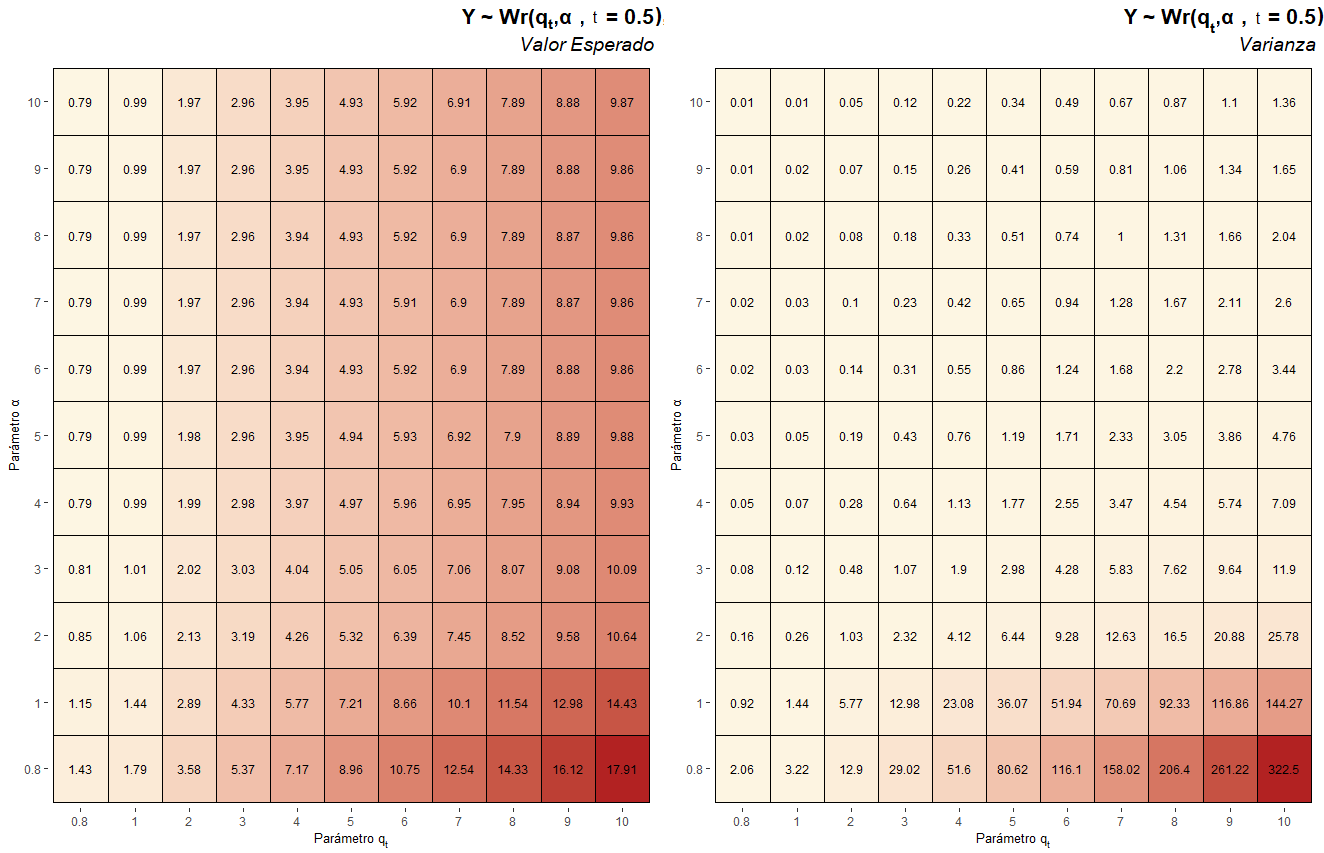
\includegraphics[width=\textwidth]{esperado}
	\caption{Valor esperado y varianza de una distribuci�n Weibull bajo la parametrizaci�n propuesta.}
	\label{espvar}
\end{figure}

	\chapter{Modelo de regresi�n cuant�lica para datos positivos}
	El presente cap�tulo tiene como objetivo especificar el modelo de regresi�n cuant�lica para datos positivos con censura intervalar. Asimismo, detallamos la estimaci�n de los par�metros desde la perspectiva de inferencia cl�sica.

	\section{Datos positivos con censura intervalar}

	Siguiendo la definici�n expuesta en \cite{peto:p}, definimos a $Y$ como una variable aleatoria con una \textbf{f.d.a.} $F(Y)$. Dicha variable se entiende como \textit{censurada} si la �nica informaci�n que tenemos sobre $Y$ es que $Y$ yace en un intervalo $I$. Bajo este contexto, podemos definir una variable aleatoria $Z$ como una variable indicadora que precisa el $j$-�simo intervalo $[a_i,b_i]$ en el que se encuentra la variable $Y$. Por lo tanto, durante el proceso de recolecci�n de datos, observamos directamente la variable $Z$, mientras que la variable $Y$ es una variable latente. Para ilustrar este proceso, imaginemos un proceso de administraci�n de encuestas, en d�nde el encuestador consulta a la persona en qu� intervalo se encuentra su sueldo mensual. Esto requiere que la variable $Z$ sea una variable categ�rica, pues la persona solo indica una opci�n. Entonces, podemos definir dicha variable mediante la siguiente expresi�n:

	\begin{equation}
	Z = 
		\begin{cases}
			1, a_{1}< y < a_{2} \\
			2, a_{2} \leq Y < a_{3} \\
			3, a_{3} \leq Y < a_{4} \\
			\vdots \\
			K, a_{k} \leq Y < a_{k+1} \\
		\end{cases}
	\end{equation}

	\noindent en d�nde $a_1 < a_2 < \cdots <a_{k+1}$. Esto corresponde a los l�mites del intervalo $I$, con $a_{1}=0$ y $a_{K+1}=\infty$. La \textbf{f.d.p} de la variable observable $Z$ est� definida de la siguiente forma:
	\begin{equation} \label{eq:2}
	P\left( Z=j \right)=P\left(a_{j} \leq Y < a_{j+1} \right) = F_Y(a_j) - F_Y(a_{j+1})
	\end{equation}

	\noindent en d�nde $F_Y(\cdot)$ es la funci�n de distribuci�n acumulada de Y. La variable $Z$ que sigue la distribuci�n anteriormente mencionada est� denotada por 
\[Z \sim \text{Categ�rica}(\pi)\]

\noindent d�nde $\pi=\left( \pi_{1},\dots,\pi_{k}\right)$y $\pi_{j}=P(Z=j)$.

\section{Funci�n de verosimilitud para datos positivos con censura intervalar}

El mecanismo de censura de datos es el proceso que no nos permite observar directamente la variable $Y$, y solo nos da como resultado la variable categ�rica $Z$. Este mecanismo, dependiendo de la casu�stica, puede aportar informaci�n adicional a la regular. Es decir, el mecanismo de censura puede indicarnos cosas adicionales a que �nicamente $y$ se encuentre en el intervalo $[a_i,a_{i+1}]$. Si ello sucediese, el investigador tendr�a que tomar en cuenta estas caracter�sticas adicionales en el proceso de estimaci�n de par�metros de la funci�n de densidad de $F'(Y)$. La presente tesis asumir� que el proceso de censura no es informativo, considerando �nicamente las ideas plasmadas por \cite{gentleman:lmk}. De acuerdo a \cite{calle:oller}, un proceso de censura no informativo considera los intervalos observados fijos e ignora su aleatoreidad. Formalmente, \cite{calle:oller} indica que la condici�n para que el proceso de censura se considere no informativo es que la distribuci�n condicional de $a_{i}$ y $a_{i+1}$ dado $Y$ satisface lo siguiente:
\begin{equation*}
f_{Z|Y}(a_{i},a_{i+1}|y_{j}) = f_{Z|Y} (a_{i},a_{i+1}|y_{k}); \{(a_{i},a_{i+1}): y_{j} \in [a_{i},a_{i+1}],y_{k} \in [a_{i},a_{i+1}]\}
\end{equation*}
\noindent Esto quiere decir que dos valores espec�ficos de $Y$, que se encuentren dentro del intervalo $[a_{i},a_{i+1}]$, contienen la misma informaci�n en $Z$. Bajo este contexto, y considerando las ideas plasmadas por \cite{gentleman:lmk}, el proceso de censura que deviene en la generaci�n de la variable $Z$ es independiente del proceso generador de datos de $Y$. Por lo tanto, nuestros par�metros de inter�s, $q_t$ y $\alpha$ no son afectados por otro proceso. Bajo esta suposici�n, consideramos la veros�militud de los datos con censura intervalar (es decir, los datos directamente observables) de la forma:

\begin{equation}
	L(\theta) = \prod_{i=1}^{n} \prod_{j=1}^{k} \pi_{ij}^{\mathbb{I}(Z_{i}=j)}
\end{equation}

Considerando los resultados identificados en la ecuaci�n \ref{eq:2}, la veros�militud de la estructura latente de los datos es de la forma:

\begin{equation}
	L(\theta) = \prod_{i=1}^{n}(F_Y(a_{j+1}) - F_Y(a_{j})) 
\end{equation}

Bajo este criterio, la veros�militud solo depende de los valores extremos del intervalo $[a_j,a_{j+1}]$ y de la \textbf{f.d.a.} de la variable latente $Y$. Para hallar los puntos �ptimos de la veros�militud, utilizaremos el m�todo de optimizaci�n de Nelder-Mead, implementado en la rutina \textit{optim} del lenguaje de programaci�n R. En la siguiente secci�n, adaptaremos el 

\section{Modelo de regresi�n para datos positivos con censura intervalar}

Considerando la reparametrizaci�n expuesta en la secci�n 2, el modelo de regresi�n cuant�lica est� dado por la siguiente expresi�n:

\[Y_{i} \sim W_{r}\left( q_{t_{i}},\alpha,t \right).\]
\[g\left( q_{t_{i}} \right) = x_{i}^{T}\beta.\]

\noindent en d�nde $\beta=\left[ \beta_0,\beta_{1},\dots,\beta_{p} \right]^{T}$ y $x_{i}^{T} =\left[ 1,x_{i1},x_{i2},\dots,x_{ip}, \right]^{T}$. La funci�n $g(\cdot)$ es una funci�n de enlace estrictamente mon�tona y doblemente diferenciable. En el presente modelo, se utilizar� la funci�n de enlace logar�tmica. El par�metro $\alpha$, el par�metro $q_{t_{i}}$ y $t$ est� definido conforme la secci�n 2.2. La estimaci�n de los par�metros $\beta$ y $\alpha$ se realizar� mediante el m�todo de m�xima verosimilitud.

\subsection{Funci�n de verosimilitud}
Consideramos que solo conocemos que $Y_{i}$ se encuentra en un intervalo de $K$ posibles intervalos de la forma $[a_{j},a_{j+1}]$ con $a_1 < a_2 < \dots < a_{k+1}$ y que $Z_{i}=j$ denota que $Y_{i} \in [a_{j},a_{j+1}]$. Por lo tanto, considerando los resultados de la secci�n 3.1, tenemos que
\[Z_{i} \sim \text{Categ�rica}(\pi_{i}).\]
\noindent con $\pi_{i}=\left( \pi_{i1},\dots, \pi_{ik} \right)$ tal que
\begin{equation}
\pi_{ij} = F_{y}(a_{j+1}|q_{t_{i}},\alpha,x) - F_{y}\left(a_{j}|q_{t_{i}},\alpha,x \right)
\end{equation}

Entonces la funci�n de verosimilitud de las variables observadas $Z_{1},Z_{2},\dots,Z_{n}$ es dada por lo siguiente:

\[L(\theta)=\prod_{i=1}^{n}\prod_{j=1}^{k} \pi_{ij}^{1\left( Z_{i}=j \right)}.\]

Luego, considerando  [$a_{i_{j}},a_{i_{j+1}}$] como el intervalo d�nde $Y_{i}$ fue observado, podemos escribir la funci�n de verosimilitud como:

\[L\left( \theta\right)=\prod_{i=1}^{n}\left( F(a_{i_{j+1}}|q_{t_{i}},\alpha,t) - F(a_{i_{j}}|q_{t_{i}},\alpha,t) \right) \]

\[L(\theta)=\sum_{i=1}^{n} \log \left( F(a_{i_{j+1}}|q_{t_{i}},\alpha,t) - F\left( a_{i_{j}}|q_{t_{i}},\alpha,t \right) \right)\]

\[L(\theta)=\sum_{i}^{n} \log \left( \exp\left( -c(t)\left( \frac{a_{i_{j}}}{e^{x_{i}^{T}\beta}} \right)^{\alpha} - \exp\left( -c(t)\left( \frac{a_{i_{j+1}}}{e^{x_{i}^{T}\beta}} \right)^{\alpha} \right) \right) \right)\]
\noindent en d�nde $c(t)=(-log(1-t))^{\frac{1}{\alpha}}$.

Los estimadores de m�xima verosimilitud para los par�metros $\alpha$ y $\beta$ se encuentran maximizando la funci�n anteriormente expuesta. Para ello, obtenemos las gradientes de $\alpha$ y $\beta$, se exponen a continuaci�n (asumiendo que $g(\cdot)$ es la funci�n logaritmo):

\[\frac{\partial L}{\partial \alpha}=\sum_{i=1}^{n} \frac{c(t)}{(\gamma_{i})^{\alpha}(\lambda_{i_{2}}-\lambda_{i_{1}})}\left( (a_{i_{j+1}})^{\alpha} \log\left( \frac{a_{i_{j+1}}}{\gamma_{i}} \right) \lambda_{i_{2}} - (a_{i_{j}})^{\alpha} \log\left( \frac{a_{i_{j+1}}}{\gamma_{i}} \right) \lambda_{i_{1}}\right)\]

\[\frac{\partial L}{\partial \beta_{j}}=\sum_{i=1}^{n} \left(\frac{\alpha c(t) x_{ij}}{(\gamma_{i})^{\alpha}(\lambda_{i_{1}}-\lambda_{i_{2}})}\right) \left( (a_{i_{j}})^{\alpha}\lambda_{i_{1}} - (a_{i_{j+1}})^{\alpha} \lambda_{i_{2}} \right)\]
\noindent en d�nde:
\[ \gamma_{i} = \exp(\eta_{i})\]
\[ \eta_{i} = x_{i}^{T}\beta\]
\[ \lambda_{i_{1}} = \exp\left( -c(t) \left(\frac{a_{i_{j}}}{\gamma_{i}}\right)^{\alpha} \right)\]
\[ \lambda_{i_{2}} = \exp\left( -c(t) \left(\frac{a_{i_{j+1}}}{\gamma_{i}}\right)^{\alpha} \right)\]

Dichos estimadores de m�xima verosimilitud, bajo ciertas condiciones de regularidad, son consistentes (es decir, que $\hat{\theta} \rightarrow \theta$ cuando $n \rightarrow \infty$) y as�ntoticamente normales con distribuci�n:

\[\hat{\theta} \sim \mathcal{N}\left(\theta,\frac{1}{\mathcal{I}(\theta)}\right).\]

\noindent cuando $n \rightarrow \infty$. $\mathcal{I}(\theta)$ es la matriz de informaci�n de Fisher, la cual en nuestro modelo tiene la estructura:

\[
\begin{bmatrix}

\frac{\partial L(\theta)}{\partial ^{2} \alpha} & \frac{\partial L(\theta)}{\partial \alpha \partial \beta_{j}}\\

\frac{\partial L(\theta)}{\partial \alpha \partial \beta_{j}} & \frac{\partial L(\theta)}{\partial^{2}\beta_{j}}

\end{bmatrix}\]

Los errores est�ndares de cada coeficiente se estiman a trav�s de la matriz de informaci�n de Fisher observada, $\mathcal{I}(\hat{\theta})$, la cual es la matriz evaluada en los estimadores de m�xima verosimilitud \cite{casella:berg}. Los errores est�ndares corresponden a la ra�z cuadrada de cada elemento de la diagonal. Finalmente, en el marco de la inferencia cl�sica, los intervalos de confianza para cada par�metro est� definido de la forma:

\[\hat{\theta} \pm \frac{z_{1-\frac{\alpha}{2}}}{\sqrt{\mathcal{I}(\hat{\theta)}}}.\]

\noindent en d�nde $\mathcal{I}(\hat{\theta})$ corresponde a la matriz de informaci�n de Fisher observada.

\section{Simulaci�n de datos}

La presente secci�n tiene como objetivo realizar un estudio de simulaci�n en el que se eval�e el adecuado la adecuada estimaci�n del modelo propuesto. Esto comprende generar una base de datos en d�nde se tenga una variable aleatoria $Y_i \sim W_r(q_t, \alpha,t)$, la cual est� subyace la variable censurada $Z$ que sigue lo denotado en la secci�n 3.1. Asimismo, dicha base de datos contiene otras variables simuladas, las cuales actuar�n como variables independientes en un contexto de regresi�n. El objetivo principal del estudio de simulaci�n evaluar si el m�todo de estimaci�n planteado, permite recuperar adecuadamente los par�metros de regresi�n establecidos anteriormente. Los criterios sobre los cuales se analizar� la estimaci�n del modelo son: sesgo relativo, error cuadr�tico medio y cobertura.

El proceso de simulaci�n consiste en generar $5.000$ r�plicas considerando tama�os de muestra de $n=\{100, 500, 1.000\}$. Simularemos la variable respuesta $Y_{i} \sim W_r(Q_{t_{i}},\alpha,t)$ considerando 3 covariables $X_{1i},X_{2i},X_{3i}$ que ser�n simuladas como:
\[X_{1i} \sim N(2,0.25)\]
\[X_{2i} \sim Beta(2,3)\]
\[X_{3i} \sim Gamma(2,20)\]

Conforme lo mencionado en la secci�n 3.2.1, $q_{t_{i}} =  \exp(x_i^T \beta)$, en d�nde $\beta =[7, 0.3, 0.84, 2.5]^T$ y $x_{i}=(1,X_{1i},X_{2i},X_{3i})^{T}$. Por otro lado, el par�metro de dispersi�n tomar� el valor $\alpha = 2$. Finalmente, se realizar� la evaluaci�n por los cuantiles $t = [0.1, 0.2, \dots, 0.9]$.

Se asume que $Y_i \sim W_r(q_{ti}, \alpha,t)$ se observa con censura intervalar. En este estudio asumiremos que solo observamos una variable $Z$ que particiona la variable $Y_i$ en intervalos de igual amplitud, con la excepci�n del �ltimo intervalo, el cual tiene la estructura $[L_{inf}, \infty]$. Una vez generada dicha variable, se realiza el modelamiento de la variable con censura intervalar sobre las variables independientes creadas previamente. El objetivo final es, a trav�s del modelo, estimar los coeficientes $\beta$ definidos previamente.

\subsection{Implementaci�n del modelo}

La implementaci�n del modelo se realiz� a trav�s del lenguaje de programaci�n R, tomando en consideraci�n las definiciones presentadas en el cap�tulo 3 de la presente tesis. El seudoc�digo de la implementaci�n es el siguiente:

\begin{lstlisting}
Simulamos valores de las siguientes distribuciones:

Definimos los siguientes valores:
N = [100, 500, 1000]
B = [7, 0.3, 0.84, 2.5] 
Sigma = 2
t=[0.1, 0.2, 0.3, 0.4, 0.5, 0.6, 0.7, 0.8, 0.9]
M = 5000

Para cada cuantil en t:
	Para cada n en N:
		Para cada replica en M:
		1 Simular n valores de las siguientes distribuciones:
			X1 ~ Beta(2,3) 
			X2 ~ Normal(2,0.5)
			X3 ~ Gamma(2,25)
		2 Generar la funci�n de enlace:
			Qt = exp(B[1] + B[2]*X1 + B[3]*X2 + B[4]*X3)
		3 Para cada i en n:
			Simular 1 valor de la siguiente distribucion:
			Y[i] ~ W_r(Qt[i], Sigma, cuantil)
		4 Censurar la variable Y de forma intervalar tal que
			Z ~ Categorica
		5 Obtener los limites inferiores y superiores de
			cada categoria de Z
		6 Crear la base de datos simulada
			df <- [L_inf, L_sup, X1, X2, X3]
		7 Ejecutar la regresion de censura intervalar
		8 Guardar los resultados
\end{lstlisting}

Una vez generadas las simulaciones, se evalu� para cada escenario (cuantil y tama�o de muestra) lo siguiente:
\[ \hat{\text{Sesgo relativo:}} \frac{1}{M}(\hat{\theta_j} - \theta)\]
\[ \hat{\text{ECM:} \frac{1}{M}} \sum_1^M (\hat{\theta_j} - \theta)^2 \]
\[ \hat{\text{Cobertura:} \frac{1}{M}} \sum_1^M (\hat{\theta_j} - \theta)^2 \]

\noindent d�nde $\theta$ es el verdadero valor del par�metro, $\hat{\theta}_{j}$ la estimaci�n obtenida en la j-�sima r�plica y M el n�mero de r�plicas.

\subsection{Resultados}

En la tabla 3.4.1 se muestra la evaluaci�n del rendimiento del modelo de regresi�n cuant�lica con censura intervalar, de acuerdo a los criterios expuestos anteriormente. Al respecto, la evaluaci�n se realiz� sobre las 5,000 r�plicas por cada cuantil y tama�o de muestra. El m�todo de estimaci�n de los par�metros se realiz� mediante la maximizaci�n de la funci�n de log-verosimilitud. 
En relaci�n al sesgo relativo, se observa que este disminuye a lo largo de todos los par�metros en la medida que aumenta el tama�o de la muestra. Cabe resaltar que para tama�os de muestra peque�os, el par�metro $\alpha$ tiende a sobre-estimarse, no obstante esto disminuye considerablemente en la medida que el tama�o de muestra aumente.

En relaci�n a la cobertura, se observa que, para todos los tama�os de muestra, los par�metros establecidos en la secci�n precedente se encuentran aproximadamente el 95\% de las veces dentro del intervalo de confianza generado.

En relaci�n al error cuadr�tico medio, se observa que, para un tama�o de muestra peque�o, el error es considerable para todos los par�metros. No obstante, esto disminuye dr�sticamente en la medida que el tama�o de muestra aumenta.

Conforme lo mencionado anteriormente, podemos concluir que el algoritmo propuesto captura adecuadamente los par�metros del modelo de regresi�n cuant�lica con censura intervalar descrito en las secciones anteriores.

\begingroup % localize the following settings                                                                    
\setlength\tabcolsep{2pt}
\setlength\LTcapwidth{\linewidth}
\setlength\LTleft{0pt}            % default: \fill
\setlength\LTright{0pt}           % default: \fill      
% Please add the following required packages to your document preamble:
% \usepackage{multirow}
% \usepackage[table,xcdraw]{xcolor}
% If you use beamer only pass "xcolor=table" option, i.e. \documentclass[xcolor=table]{beamer}
% \usepackage{lscape}
% \usepackage{longtable}
% Note: It may be necessary to compile the document several times to get a multi-page table to line up properly
\begin{landscape}
\footnotesize
\begin{longtable}[c]{cc|c|c|c|c|c|c|c|c|c|c|c|c|c|c|c}
\cline{3-17}
\multicolumn{1}{l}{} &
  \multicolumn{1}{l|}{} &
  \multicolumn{5}{c|}{\cellcolor[HTML]{9B9B9B}\textbf{Cobertura del Intervalo de confianza}} &
  \multicolumn{5}{c|}{\cellcolor[HTML]{9B9B9B}\textbf{Error Cuadr�tico Medio}} &
  \multicolumn{5}{c|}{\cellcolor[HTML]{9B9B9B}\textbf{Sesgo}} \\ \cline{3-17} 
\endfirsthead
%
\endhead
%
\multicolumn{1}{l}{} &
  \multicolumn{1}{l|}{} &
  \cellcolor[HTML]{C0C0C0}\textbf{$\beta_0$} &
  \cellcolor[HTML]{C0C0C0}\textbf{$\beta_1$} &
  \cellcolor[HTML]{C0C0C0}\textbf{$\beta_2$} &
  \cellcolor[HTML]{C0C0C0}\textbf{$\beta_3$} &
  \cellcolor[HTML]{C0C0C0}\textbf{$\alpha$} &
  \cellcolor[HTML]{C0C0C0}\textbf{$\beta_0$} &
  \cellcolor[HTML]{C0C0C0}\textbf{$\beta_1$} &
  \cellcolor[HTML]{C0C0C0}\textbf{$\beta_2$} &
  \cellcolor[HTML]{C0C0C0}\textbf{$\beta_3$} &
  \cellcolor[HTML]{C0C0C0}\textbf{$\alpha$} &
  \cellcolor[HTML]{C0C0C0}\textbf{$\beta_0$} &
  \cellcolor[HTML]{C0C0C0}\textbf{$\beta_1$} &
  \cellcolor[HTML]{C0C0C0}\textbf{$\beta_2$} &
  \cellcolor[HTML]{C0C0C0}\textbf{$\beta_3$} &
  \cellcolor[HTML]{C0C0C0}\textbf{$\alpha$} \\ \hline
\multicolumn{1}{|c|}{\cellcolor[HTML]{9B9B9B}} &
  \cellcolor[HTML]{C0C0C0}\textbf{$\tau = 0.1$} &
  93.90\% &
  94.14\% &
  94.04\% &
  94.56\% &
  94.90\% &
  0.3005 &
  0.0595 &
  0.0982 &
  0.9626 &
  0.0561 &
  0.0319 &
  0.0034 &
  -0.0007 &
  0.0332 &
  \multicolumn{1}{c|}{0.1016} \\ \cline{2-17} 
\multicolumn{1}{|c|}{\cellcolor[HTML]{9B9B9B}} &
  \cellcolor[HTML]{C0C0C0}\textbf{$\tau = 0.2$} &
  93.62\% &
  93.96\% &
  94.22\% &
  93.92\% &
  94.82\% &
  0.2843 &
  0.0591 &
  0.1004 &
  0.9800 &
  0.0570 &
  0.0261 &
  0.0000 &
  0.0020 &
  0.0071 &
  \multicolumn{1}{c|}{0.1009} \\ \cline{2-17} 
\multicolumn{1}{|c|}{\cellcolor[HTML]{9B9B9B}} &
  \cellcolor[HTML]{C0C0C0}\textbf{$\tau = 0.3$} &
  93.88\% &
  93.84\% &
  94.36\% &
  93.36\% &
  94.66\% &
  0.2763 &
  0.0595 &
  0.0989 &
  1.0171 &
  0.0531 &
  0.0134 &
  0.0008 &
  0.0045 &
  -0.0033 &
  \multicolumn{1}{c|}{0.0921} \\ \cline{2-17} 
\multicolumn{1}{|c|}{\cellcolor[HTML]{9B9B9B}} &
  \cellcolor[HTML]{C0C0C0}\textbf{$\tau = 0.4$} &
  94.22\% &
  94.42\% &
  94.48\% &
  93.88\% &
  94.54\% &
  0.2643 &
  0.0577 &
  0.0952 &
  0.9685 &
  0.0582 &
  0.0116 &
  0.0023 &
  -0.0102 &
  -0.0112 &
  \multicolumn{1}{c|}{0.1060} \\ \cline{2-17} 
\multicolumn{1}{|c|}{\cellcolor[HTML]{9B9B9B}} &
  \cellcolor[HTML]{C0C0C0}\textbf{$\tau = 0.5$} &
  93.78\% &
  94.24\% &
  93.98\% &
  93.86\% &
  94.18\% &
  0.2711 &
  0.0587 &
  0.0986 &
  0.9897 &
  0.0597 &
  -0.0017 &
  0.0029 &
  -0.0013 &
  0.0050 &
  \multicolumn{1}{c|}{0.1082} \\ \cline{2-17} 
\multicolumn{1}{|c|}{\cellcolor[HTML]{9B9B9B}} &
  \cellcolor[HTML]{C0C0C0}\textbf{$\tau = 0.6$} &
  94.62\% &
  94.92\% &
  94.20\% &
  93.62\% &
  94.18\% &
  0.2577 &
  0.0575 &
  0.0992 &
  1.0313 &
  0.0578 &
  -0.0027 &
  -0.0007 &
  0.0008 &
  0.0497 &
  \multicolumn{1}{c|}{0.1024} \\ \cline{2-17} 
\multicolumn{1}{|c|}{\cellcolor[HTML]{9B9B9B}} &
  \cellcolor[HTML]{C0C0C0}\textbf{$\tau = 0.7$} &
  93.68\% &
  93.34\% &
  93.98\% &
  94.48\% &
  94.92\% &
  0.2752 &
  0.0623 &
  0.0987 &
  0.9527 &
  0.0566 &
  -0.0091 &
  0.0031 &
  -0.0044 &
  -0.0034 &
  \multicolumn{1}{c|}{0.1039} \\ \cline{2-17} 
\multicolumn{1}{|c|}{\cellcolor[HTML]{9B9B9B}} &
  \cellcolor[HTML]{C0C0C0}\textbf{$\tau = 0.8$} &
  94.44\% &
  93.82\% &
  94.46\% &
  94.00\% &
  94.78\% &
  0.2687 &
  0.0610 &
  0.0959 &
  0.9666 &
  0.0572 &
  -0.0170 &
  0.0020 &
  -0.0026 &
  0.0112 &
  \multicolumn{1}{c|}{0.1044} \\ \cline{2-17} 
\multicolumn{1}{|c|}{\multirow{-9}{*}{\cellcolor[HTML]{9B9B9B}\textbf{$ n = 100$}}} &
  \cellcolor[HTML]{C0C0C0}\textbf{$\tau = 0.9$} &
  93.66\% &
  93.00\% &
  94.50\% &
  93.94\% &
  94.50\% &
  0.2726 &
  0.0622 &
  0.0970 &
  0.9568 &
  0.0585 &
  -0.0277 &
  0.0047 &
  0.0013 &
  -0.0150 &
  \multicolumn{1}{c|}{0.1081} \\ \hline
\multicolumn{1}{|c|}{\cellcolor[HTML]{9B9B9B}} &
  \cellcolor[HTML]{C0C0C0}\textbf{$\tau = 0.1$} &
  94.28\% &
  94.54\% &
  94.76\% &
  94.34\% &
  95.22\% &
  0.0580 &
  0.0113 &
  0.0195 &
  0.1928 &
  0.0091 &
  0.0163 &
  -0.0026 &
  -0.0018 &
  0.0157 &
  \multicolumn{1}{c|}{0.0266} \\ \cline{2-17} 
\multicolumn{1}{|c|}{\cellcolor[HTML]{9B9B9B}} &
  \cellcolor[HTML]{C0C0C0}\textbf{$\tau = 0.2$} &
  95.00\% &
  95.36\% &
  94.42\% &
  94.40\% &
  94.88\% &
  0.0514 &
  0.0107 &
  0.0193 &
  0.1850 &
  0.0094 &
  0.0127 &
  -0.0021 &
  -0.0016 &
  -0.0129 &
  \multicolumn{1}{c|}{0.0251} \\ \cline{2-17} 
\multicolumn{1}{|c|}{\cellcolor[HTML]{9B9B9B}} &
  \cellcolor[HTML]{C0C0C0}\textbf{$\tau = 0.3$} &
  94.66\% &
  94.52\% &
  94.56\% &
  93.82\% &
  93.98\% &
  0.0515 &
  0.0112 &
  0.0190 &
  0.1989 &
  0.0098 &
  0.0015 &
  0.0035 &
  -0.0015 &
  -0.0264 &
  \multicolumn{1}{c|}{0.0257} \\ \cline{2-17} 
\multicolumn{1}{|c|}{\cellcolor[HTML]{9B9B9B}} &
  \cellcolor[HTML]{C0C0C0}\textbf{$\tau = 0.4$} &
  95.18\% &
  94.82\% &
  94.82\% &
  94.54\% &
  94.22\% &
  0.0492 &
  0.0111 &
  0.0185 &
  0.1876 &
  0.0095 &
  -0.0016 &
  0.0028 &
  -0.0008 &
  -0.0051 &
  \multicolumn{1}{c|}{0.0262} \\ \cline{2-17} 
\multicolumn{1}{|c|}{\cellcolor[HTML]{9B9B9B}} &
  \cellcolor[HTML]{C0C0C0}\textbf{$\tau = 0.5$} &
  94.44\% &
  94.44\% &
  95.20\% &
  94.96\% &
  94.56\% &
  0.0524 &
  0.0115 &
  0.0187 &
  0.1783 &
  0.0094 &
  0.0019 &
  0.0003 &
  -0.0017 &
  -0.0019 &
  \multicolumn{1}{c|}{0.0252} \\ \cline{2-17} 
\multicolumn{1}{|c|}{\cellcolor[HTML]{9B9B9B}} &
  \cellcolor[HTML]{C0C0C0}\textbf{$\tau = 0.6$} &
  94.22\% &
  94.50\% &
  94.98\% &
  94.70\% &
  94.62\% &
  0.0519 &
  0.0114 &
  0.0186 &
  0.1813 &
  0.0096 &
  -0.0013 &
  0.0016 &
  -0.0011 &
  -0.0055 &
  \multicolumn{1}{c|}{0.0257} \\ \cline{2-17} 
\multicolumn{1}{|c|}{\cellcolor[HTML]{9B9B9B}} &
  \cellcolor[HTML]{C0C0C0}\textbf{$\tau = 0.7$} &
  94.40\% &
  95.12\% &
  94.40\% &
  94.54\% &
  94.50\% &
  0.0503 &
  0.0111 &
  0.0193 &
  0.1871 &
  0.0095 &
  0.0015 &
  -0.0007 &
  -0.0022 &
  -0.0048 &
  \multicolumn{1}{c|}{0.0245} \\ \cline{2-17} 
\multicolumn{1}{|c|}{\cellcolor[HTML]{9B9B9B}} &
  \cellcolor[HTML]{C0C0C0}\textbf{$\tau = 0.8$} &
  94.20\% &
  94.40\% &
  94.68\% &
  93.70\% &
  94.70\% &
  0.0516 &
  0.0114 &
  0.0190 &
  0.1964 &
  0.0096 &
  -0.0022 &
  0.0009 &
  -0.0011 &
  -0.0271 &
  \multicolumn{1}{c|}{0.0258} \\ \cline{2-17} 
\multicolumn{1}{|c|}{\multirow{-9}{*}{\cellcolor[HTML]{9B9B9B}\textbf{$ n = 500$}}} &
  \cellcolor[HTML]{C0C0C0}\textbf{$\tau = 0.9$} &
  94.60\% &
  95.00\% &
  94.70\% &
  94.12\% &
  94.82\% &
  0.0489 &
  0.0109 &
  0.0191 &
  0.1867 &
  0.0093 &
  -0.0063 &
  0.0004 &
  0.0036 &
  -0.0033 &
  \multicolumn{1}{c|}{0.0245} \\ \hline
\multicolumn{1}{|c|}{\cellcolor[HTML]{9B9B9B}} &
  \cellcolor[HTML]{C0C0C0}\textbf{$\tau = 0.1$} &
  94.66\% &
  94.42\% &
  94.10\% &
  94.42\% &
  95.08\% &
  0.0287 &
  0.0056 &
  0.0099 &
  0.0956 &
  0.0044 &
  0.0100 &
  -0.0016 &
  -0.0017 &
  0.0078 &
  \multicolumn{1}{c|}{0.0146} \\ \cline{2-17} 
\multicolumn{1}{|c|}{\cellcolor[HTML]{9B9B9B}} &
  \cellcolor[HTML]{C0C0C0}\textbf{$\tau = 0.2$} &
  94.74\% &
  95.44\% &
  94.60\% &
  93.94\% &
  94.94\% &
  0.0262 &
  0.0054 &
  0.0097 &
  0.0974 &
  0.0044 &
  0.0016 &
  0.0026 &
  -0.0025 &
  -0.0181 &
  \multicolumn{1}{c|}{0.0129} \\ \cline{2-17} 
\multicolumn{1}{|c|}{\cellcolor[HTML]{9B9B9B}} &
  \cellcolor[HTML]{C0C0C0}\textbf{$\tau = 0.3$} &
  95.12\% &
  94.96\% &
  94.40\% &
  92.60\% &
  94.66\% &
  0.0261 &
  0.0055 &
  0.0096 &
  0.1042 &
  0.0047 &
  0.0025 &
  0.0008 &
  -0.0008 &
  -0.0188 &
  \multicolumn{1}{c|}{0.0110} \\ \cline{2-17} 
\multicolumn{1}{|c|}{\cellcolor[HTML]{9B9B9B}} &
  \cellcolor[HTML]{C0C0C0}\textbf{$\tau = 0.4$} &
  94.92\% &
  94.62\% &
  94.44\% &
  94.64\% &
  95.52\% &
  0.0253 &
  0.0055 &
  0.0097 &
  0.0930 &
  0.0044 &
  0.0029 &
  -0.0008 &
  0.0007 &
  0.0014 &
  \multicolumn{1}{c|}{0.0130} \\ \cline{2-17} 
\multicolumn{1}{|c|}{\cellcolor[HTML]{9B9B9B}} &
  \cellcolor[HTML]{C0C0C0}\textbf{$\tau = 0.5$} &
  95.34\% &
  94.74\% &
  94.26\% &
  94.88\% &
  95.32\% &
  0.0251 &
  0.0055 &
  0.0094 &
  0.0897 &
  0.0045 &
  0.0028 &
  -0.0008 &
  -0.0008 &
  -0.0076 &
  \multicolumn{1}{c|}{0.0133} \\ \cline{2-17} 
\multicolumn{1}{|c|}{\cellcolor[HTML]{9B9B9B}} &
  \cellcolor[HTML]{C0C0C0}\textbf{$\tau = 0.6$} &
  94.98\% &
  94.86\% &
  94.48\% &
  94.90\% &
  94.98\% &
  0.0245 &
  0.0054 &
  0.0095 &
  0.0889 &
  0.0045 &
  -0.0026 &
  0.0022 &
  -0.0027 &
  -0.0044 &
  \multicolumn{1}{c|}{0.0143} \\ \cline{2-17} 
\multicolumn{1}{|c|}{\cellcolor[HTML]{9B9B9B}} &
  \cellcolor[HTML]{C0C0C0}\textbf{$\tau = 0.7$} &
  94.48\% &
  94.82\% &
  94.22\% &
  94.08\% &
  94.92\% &
  0.0252 &
  0.0056 &
  0.0097 &
  0.0963 &
  0.0046 &
  -0.0016 &
  0.0003 &
  0.0020 &
  -0.0058 &
  \multicolumn{1}{c|}{0.0122} \\ \cline{2-17} 
\multicolumn{1}{|c|}{\cellcolor[HTML]{9B9B9B}} &
  \cellcolor[HTML]{C0C0C0}\textbf{$\tau = 0.8$} &
  94.56\% &
  94.54\% &
  94.66\% &
  93.46\% &
  94.58\% &
  0.0256 &
  0.0058 &
  0.0094 &
  0.0997 &
  0.0046 &
  -0.0055 &
  0.0028 &
  -0.0018 &
  -0.0086 &
  \multicolumn{1}{c|}{0.0119} \\ \cline{2-17} 
\multicolumn{1}{|c|}{\multirow{-9}{*}{\cellcolor[HTML]{9B9B9B}\textbf{$ n = 1000$}}} &
  \cellcolor[HTML]{C0C0C0}\textbf{$\tau = 0.9$} &
  95.06\% &
  94.66\% &
  94.84\% &
  95.16\% &
  94.24\% &
  0.0244 &
  0.0055 &
  0.0094 &
  0.0894 &
  0.0047 &
  -0.0022 &
  0.0000 &
  -0.0014 &
  -0.0022 &
  \multicolumn{1}{c|}{0.0143} \\ \hline
\caption{Evaluaci�n del estudio de simulaci�n}
\end{longtable}
\end{landscape}

\chapter{Aplicaci�n en datos reales}

El presente cap�tulo presenta una aplicaci�n del modelo de regresi�n cuant�lica para datos intervalares en un conjunto de datos reales. Para tal fin, se utilizar� la Encuesta Nacional de Satisfacci�n de Usuarios del Aseguramiento Universal en Salud (ENSUSALUD) la cual ha sido generada por el Instituto Nacional de Estad�stica e Inform�tica del Per� (INEI). En dicha aplicaci�n, se evaluar� el efecto de cada covariable en la variable respuesta a lo largo de todos los cuantiles. 

\section{ENSUSALUD 2015}
Conforme el Convenio de Cooperaci�n Interinstitucional N� 017-2013-INEI, el INEI y la Superintendencia Nacional de Aseguramiento en Salud (SUNASA) acordaron en implementar y ejecutar la encuesta de satisfacci�n en salud el a�o 2015. Dicha encuesta es una investigaci�n estad�stica, cuyo objetivo es <<evaluar el grado de satisfacci�n de los usuarios internos y externos de los servicios de salud>> \cite{inei:ensusalud}. Al respecto, dicha encuesta comprende como unidad muestral a los usuarios de consulta externa, b�ticas y farmacias, seguros, y profesionales de la salud. Los usuarios y profesionales han sido atendidos o forman parte del conjunto de establecimientos del Ministerio de Salud (MINSA), Seguro Social de Salud (EsSalud), Cl�nicas privadas y Establecimientos de Sanidad de las Fuerzas Armadas y Policiales.

En relaci�n al dise�o muestral de la encuesta, esta consiste en un muestreo probabil�stico poliet�pico, cuya unidad primaria de muestreo (UPM) est� constituida cada establecimiento de salud de las redes hospitalarias del MINSA, EsSalud, cl�nicas privadas y Establecimientos de las Fuerzas Armadas y Policiales. La unidad secundaria de muestreo (USM) consiste en los usuarios elegibles y profesionales de la salud. En resumen, la investigaci�n estad�stica tiene el siguiente alcance:

\begin{itemize}
	\item \textbf{Cobertura geogr�fica:} Los 24 departamentos del Per� y 181 establecimientos de salud del MINSA, EsSalud, Sanidades y establecimientos privados.
	\item \textbf{Unidad de an�lisis:} La unidad muestral comprende a los siguientes:
		\begin{itemize}
			\item Usuarios de Consulta Externa.
			\item Usuarios en Boticas y Farmacias.
			\item Usuarios en Unidades de Seguros.
			\item Profesionales de la Salud.
		\end{itemize}
	\item \textbf{Niveles de inferencia:} Nacional y dirigida a cada una de las unidades de an�lisis.
\end{itemize}

\section{Base de datos}
Para prop�sitos de la aplicaci�n, se utiliz� la encuesta ejecutada a profesionales de la salud (enfermer�a y personal m�dico). Esta encuesta se realiz� a 5,067 profesionales en el a�o 2015 \cite{inei:ensusalud}, y tiene como objetivo <<conocer caracter�sticas del personal relacionados a formaci�n acad�mica, actividad laboral, satisfacci�n con el trabajo, estr�s laboral y conocimiento referido a la SUNASA>>. Considerando las respuestas v�lidas relacionadas al sueldo de los profesionales, tenemos 4,973 profesionales materia de an�lisis, entre m�dicos/as y enfermeros/as. El an�lisis final se realizar� sobre los m�dicos/as (2,154 profesionales). Esta base de datos ha sido estudiada previamente por \cite{salyrosas:bayes}, quienes evaluaron la disparidad de sueldos entre profesionales varones y mujeres. Al respecto, dicho estudio estableci� una regresi�n de censura intervalar, la cual ha sido extendida a una regresi�n cuant�lica en la presente tesis.


\section{Conjunto de Variables}

De dicha base de datos, se utilizaron las siguientes variables:

\begin{itemize}
	\itemsep0em
	\item \textbf{Caracter�sticas del establecimiento de salud:} (i) Tipo de instituci�n del establecimiento.
	\item \textbf{Caracterizaci�n del profesional de salud:} (i) Profesi�n espec�fica del personal de salud.
	\item \textbf{Formaci�n acad�mica del profesional de salud:} (i) Si el profesional cuenta con especialidad o no.
	\item \textbf{Actividad laboral del profesional de salud:} (i) A�os de experiencia en el sector salud; (ii) Si el profesional realiza labor asistencial en otra instituci�n; (iii) Si el profesional realiza labor docente remunerada; (iv) Cantidad de horas laboradas semanalmente por el profesional de salud; \textbf{(v) El ingreso mensual (censurado intervalarmente) del profesional de salud}
\end{itemize}

\section{Resultados}

Se ajust� el modelo de regresi�n cuant�lica para datos con censura intervalar a dichos datos. Considerando la funci�n de enlace logar�tmica, se estim� los par�metros $\beta$ y $\alpha$. Los resultados de las regresiones, as� como el intervalo de confianza asociado a cada par�metro, se encuentran en la figura \ref{med:efectos}.

La categor�a de referencia para el presente estudio es un m�dico hombre, que trabaja en el instituto MINSA-GR y cuenta con especialidad (C2P13), realiza labor asistencial en otra instituci�n, y realiza labor docente remunerada (C2P26). Al respecto, se observa lo siguiente:
\begin{itemize}
	\item Para cada uno de los cuantiles de la variable respuesta, se observa que una m�dico mujer tendr�a un decremento entre $\beta = [-0.05, -0.11]; e^{\beta}-1 = [-0.11,-0.06]$ en relaci�n a sus pares varones. El efecto se acent�a en mayor medida en el cuantil 0.9 de la variable respuesta.
	\item Para ciertos cuantiles, y tomando en cuenta la categor�a de referencia, cambiar de la instituci�n MINSA-GR a las instituciones FF.AA. / PN o Cl�nicas Privadas tiene como consecuencia un decremento en el sueldo. No obstante, se observa que ello podr�a no tener efecto para estos cuantiles, pues los intervalos de confianza contienen el 0.
	\item A lo largo de todos los cuantiles de la variable respuesta, existe un marcado efecto negativo en tanto el m�dico no realice labor asistencial en otra instituci�n o no realice labor docente remunerada.
\end{itemize}

\begin{figure}
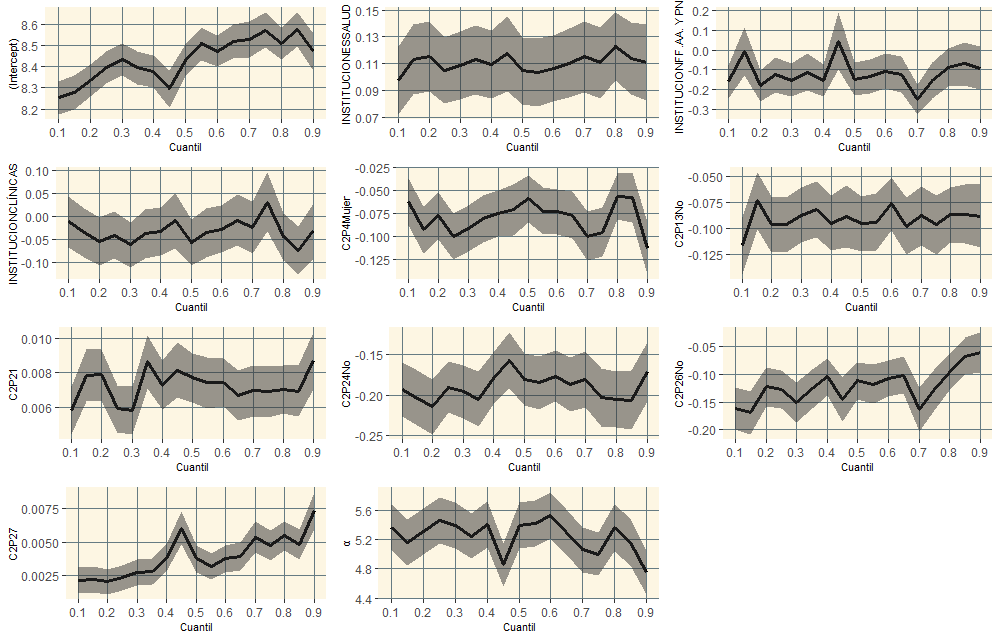
\includegraphics[width=\textwidth]{figuras/efectos_med.png}
\caption{Efectos de las covariables sobre los cuantiles del sueldo de los m�dicos/as}
\label{med:efectos}

\end{figure}

\chapter{Conclusiones}
\section{Conclusiones}

Los datos con censura intervalar presentan retos en el proceso de modelamiento de datos, pues la no-observabilidad de los mismos requiere adaptar los procesos de inferencia cl�sica a esta estructura. Ante ello, la presente tesis estudi� un modelo de regresi�n cuant�lica para datos con censura intervalar, en base a los estudios realizados anteriormente por \cite{peto:p}, \cite{gentleman:lmk} y \cite{koenker:kk}. Dicho modelo de regresi�n es param�trico, asumiendo que la variable latente sigue una distribuci�n de Weibull, la cual fue reparametrizada para estudiar los efectos de las covariables en distintos cuantiles de la variable respuesta.

Para evaluar el modelo propuesto, se realiz� un estudio de simulaci�n para diversos cuantiles y distintos tama�os de muestras. Se observ� que el estimador propuesto captura apropiadamente los par�metros poblacionales, y que el sesgo y error cuadr�tico medio se redujo en la medida que aument� el n�mero de observaciones. La cobertura de los intervalos de confianza fue apropiada en todos los tama�os de muestra.

Finalmente, se aplic� el modelo de regresi�n a datos de la Encuesta Nacional de Satisfacci�n de Usuarios en Salud (ENSUSALUD) 2015. En dicha encuesta, el sueldo de los profesionales de salud (m�dicos/as y enfermeros/as) se censur� desde el proceso de recolecci�n de datos. Atendiendo al estudio realizado por \cite{salyrosas:bayes}, la presente tesis extiende el modelo de regresi�n de censura intervalar expuesto a un modelo de regresi�n cuant�lica. El presente modelo permiti� analizar los factores de las covariables en relaci�n al sueldo de dichos profesionales, por cada uno de los cuantiles de la variable respuesta.

\section{Sugerencias para investigaciones futuras}
\begin{itemize}
	\item Establecer una metodolog�a de m�xima verosimilitud que tome en cuenta el dise�o muestral a trav�s los pesos muestrales de la encuesta realizada. Asimismo, proponer m�todos para la estimaci�n de los errores est�ndar atendiendo esta estructura.
	\item Proponer un modelo de regresi�n cuant�lica con censura intervalar bajo inferencia bayesiana, tomando en consideraci�n los m�todos expuestos en la presente tesis.
\end{itemize}

\chapter{Ap�ndice}

\section{Pseudoc�digo de la simulaci�n}
\label{seudo}

\begin{lstlisting}
Simulamos valores de las siguientes distribuciones:

Definimos los siguientes valores:
N = [100, 500, 1000]
B = [7, 0.3, 0.84, 2.5] 
Sigma = 2
t=[0.1, 0.2, 0.3, 0.4, 0.5, 0.6, 0.7, 0.8, 0.9]
M = 5000

Para cada cuantil en t:
	Para cada n en N:
		Para cada replica en M:
		1 Simular n valores de las siguientes distribuciones:
			X1 ~ Beta(2,3) 
			X2 ~ Normal(2,0.5)
			X3 ~ Gamma(2,25)
		2 Generar la funci�n de enlace:
			Qt = exp(B[1] + B[2]*X1 + B[3]*X2 + B[4]*X3)
		3 Para cada i en n:
			Simular 1 valor de la siguiente distribucion:
			Y[i] ~ W_r(Qt[i], Sigma, cuantil)
		4 Censurar la variable Y de forma intervalar tal que
			Z ~ Categorica
		5 Obtener los limites inferiores y superiores de
			cada categoria de Z
		6 Crear la base de datos simulada
			df <- [L_inf, L_sup, X1, X2, X3]
		7 Ejecutar la regresion de censura intervalar
		8 Guardar los resultados
\end{lstlisting}

\section{Aplicaci�n en R}

\begin{lstlisting}[basicstyle=\tiny]
library(gamlss)
library(gamlss.cens)
library(haven)
library(tidyverse)
library(BB)
library(matrixStats)
library(gridExtra)
library(numDeriv)
library(pracma)
library(ucminf)
library(nloptr)
library(ggthemes)

gen.cens(family="WEI3",type="interval")

Ct = function(alpha, tau){
  (-log(1-tau))^(1/alpha)
}
F_Wr = function(Y,Qt,alpha,tau){
  B = Qt/Ct(alpha,tau)
  pweibull(Y,shape=alpha,scale=B)
}
Qt_b = function(betas, df){
  Qt_c = exp(as.matrix(df[['matriz.diseno']]) %*% betas)
  return(Qt_c)
}
Qt_a = function(betas, df){
  Qt_c = exp(as.matrix(df) %*% betas)
  return(Qt_c)
}
Rand_Wr = function(n,Qt,alpha,tau){
  B = Qt/Ct(alpha,tau)
  rweibull(n,shape = alpha,scale = B)
}
Simulation = function(n){
  X1 = rnorm(n,2,0.25)
  X2 = rbeta(n,2,3)
  X3 = rgamma(n,2,20)
  df = data.frame(X1 = X1, X2 = X2, X3 = X3)
  return(df)
}
DF_Simulation = function(df,betas,alpha,tau){
  M = dim(df)[1]
  design_matrix = model.matrix(~ . ,df)
  Qt_i = Qt_a(betas,design_matrix)
  Y = c()
  for (j in 1:M) {
    Y=rbind(Y,Rand_Wr(1,Qt_i[j],alpha,tau))
  }
  min_Y = floor(min(Y))
  if (min_Y==0) {
    min_Y <- 0.01
  }
  Q8_Y = round(quantile(Y,0.8),2)
  interval = round((Q8_Y-min_Y) / 6,2)
  seq_interv = c(seq(min_Y,Q8_Y,interval),Inf)
  Ls = c()
  for (u in 1:length(Y)) {
    for (n in 1:length(seq_interv)) {
      if (Y[u] <seq_interv[n]) {
        Ls[u] = seq_interv[n]
        break
      }}}
  Li = c()
  for (p in 1:length(Y)) {
    for (w in 1:length(seq_interv)) {
      if (Y[p] > rev(seq_interv)[w]) {
        Li[p] = rev(seq_interv)[w]
        break
      }}}
  F_df = cbind(data.frame(Li = round(Li,2), Ls = round(Ls,2)),df)
  return(F_df)
}
data_mgmt = function(data,li,lf){
  df_inf = data[,li]
  df_sup = data[,lf]
  covar = as.data.frame(data[,-c(li,lf)])
  covar = model.matrix(~. , covar)
  lista = list(lim.inferior = df_inf, lim.superior = df_sup, matriz.diseno = covar)
  return(lista)
}
likelihood = function(param,betas,df,tau){
  n = length(param)-1
  for(i in 1:n){betas[i]=param[i]}
  alpha = param[length(param)]
  Qt_i = Qt_b(betas,df)
  -sum(log(F_Wr(df[['lim.superior']],Qt_i,alpha,tau)
       -F_Wr(df[['lim.inferior']],Qt_i,alpha,tau)))
}
reg_Wr = function(data,li,lf,tau,param){
  df = data_mgmt(data,li,lf)
  Bs = as.matrix(rep(0,ncol(df[['matriz.diseno']])))
  fit_mv = nloptr(x0 = param,eval_f = likelihood, betas=Bs, df=df, tau=tau,
  opts = list("algorithm"=c("NLOPT_LN_SBPLX"),maxeval = 400)
  ,lb = c(-Inf,-Inf,-Inf,-Inf,-Inf,-Inf,-Inf,-Inf,-Inf,-Inf,-Inf)
  ,ub=c(Inf,Inf,Inf,Inf,Inf,Inf,Inf,Inf,Inf,Inf,Inf))
  print(fit_mv$message)
  fit_mv$hessian = pracma::hessian(x0 = fit_mv$solution,f = likelihood,betas=Bs,df=df,tau=tau)
  return(fit_mv)
}

lancet <- function(int){
  temp <- tempfile()
  download.file("http://iinei.inei.gob.pe/iinei/srienaho/descarga/SPSS/447-Modulo552.zip", temp)
  salud <- read_sav(unz(temp, "447-Modulo552/04_C2_CAPITULOS.sav"))
  unlink(temp)
  
  salud <- salud[salud$C2P28 != 7,]
  
  salud$C2P26
  
  ### Pre-procesamiento ###
  variables <- c("INSTITUCION","C2P4","C2P13","C2P21","C2P24","C2P26","C2P28","C2P1","C2P27")
  
  newsalud <- salud[variables]
  
  newsalud$li <- NULL
  newsalud$ls <- NULL
  newsalud$li <- ifelse(newsalud$C2P28 == 1, 850,
                        ifelse(newsalud$C2P28 == 2, 1000,
                               ifelse(newsalud$C2P28 == 3, 2001,
                                      ifelse(newsalud$C2P28 == 4, 3001,
                                             ifelse(newsalud$C2P28 == 5, 4001, 5001)))))
  newsalud$lf <- ifelse(newsalud$C2P28 == 1, 999,
                        ifelse(newsalud$C2P28 == 2, 2000,
                               ifelse(newsalud$C2P28 == 3, 3000,
                                      ifelse(newsalud$C2P28 == 4, 4000,
                                             ifelse(newsalud$C2P28 == 5, 5000, Inf)))))
  
  newsalud <- newsalud %>% select(-C2P28)
  
  newsalud$INSTITUCION <- factor(newsalud$INSTITUCION,labels=names(attr(newsalud$INSTITUCION,"labels")))
  newsalud$C2P4 <- factor(newsalud$C2P4,labels = names(attr(newsalud$C2P4,"labels")))
  newsalud$C2P13 <- factor(newsalud$C2P13, labels=names(attr(newsalud$C2P13,"labels")))
  newsalud$C2P21 <- as.integer(newsalud$C2P21)
  newsalud$C2P24 <- factor(newsalud$C2P24, labels = names(attr(newsalud$C2P24,"labels")))
  newsalud$C2P26 <- factor(newsalud$C2P26, labels = names(attr(newsalud$C2P26,"labels")))
  newsalud$C2P1 <- factor(newsalud$C2P1, labels = names(attr(newsalud$C2P1,"labels")))
  newsalud$C2P27 <- as.integer(newsalud$C2P27)
  
  newsalud_enf <- newsalud[newsalud$C2P1 =="Enfermero/a" ,]
  newsalud_enf <- subset(newsalud_enf, select = -C2P1)
  newsalud_enf <- as.data.frame(newsalud_enf)
  
  newsalud_med <- newsalud[newsalud$C2P1 == "M�dico",]
  newsalud_med <- subset(newsalud_med, select = -C2P1)
  newsalud_med <- as.data.frame(newsalud_med)
  if (int == 1) {
    return(newsalud_enf)  
  }
  if (int ==2) {
    return(newsalud_med)
  }
  if (int ==3) {
    newsalud_total <- as.data.frame(subset(newsalud,select = -C2P1))
    return(newsalud_total)
  }
}

#### Simulaci�n ####

L = 5000
n = c(100,500,1000)
betas_sim = c(7,0.3,0.84,2.5)
alpha_sim = 2
tau_sim = seq(0.1,0.9,0.1)

sim_list= list(n100 = list(), n500 = list(), n1000 = list())

for (j in 1:length(n)) {
  for (k in 1:length(tau_sim)) {
    for (p in 1:L) {
      sim = Simulation(n[j])
      df_sim = DF_Simulation(sim,betas_sim,alpha_sim,tau_sim[k])
      m0 = gamlss(Surv(Li,Ls,type="interval2")~.,family = WEI3ic,data = na.omit(df_sim))
      init = as.vector(c(coef(m0),m0$sigma.coefficients))
      sim_list[[j]] = append(sim_list[[j]],list(reg_Wr(data = df_sim,
                       li = 1,lf = 2,tau = tau_sim[k],param = init)))
    }
  }
}

se_calc <- function(lista) {
  ic_contain <- matrix(nrow=0,ncol=5)
  for (k in 1:length(lista)) {
    little_t <- lista[[k]]
    ic <- rbind( little_t$par - qnorm(0.975) * sqrt(diag(solve(little_t$hessian))),
                 little_t$par + qnorm(0.975) * sqrt(diag(solve(little_t$hessian))))
    ic_contain <- rbind(ic_contain,cbind(between(betas_sim[1],left = ic[1,1],right = ic[2,1]),
                        between(betas_sim[2],left = ic[1,2],right = ic[2,2]),
                        between(betas_sim[3],left = ic[1,3],right = ic[2,3]),
                        between(betas_sim[4],left = ic[1,4],right = ic[2,4]),
                        between(alpha_sim,left = ic[1,5],right = ic[2,5])))
  }
  final_df <- as.matrix(t(colSums(ic_contain)/length(lista)))
  return(final_df)
}

final_database <- matrix(nrow=0,ncol=5)
seq_t <- seq(1,8,1);seq_t

for (j in 1:length(n)) {
  df <- sim_list[[j]]
  actual_t <- df[1:5000*seq_t[1]]
  vf_df <- se_calc(actual_t)
  rownames(vf_df) <- paste("n_",n[j],sep="")
  final_database <- rbind(final_database,vf_df)
  
  for (l in 1:length(seq_t)) {
   actual_t <-  df[(5000*seq_t[l]+1):(5000*(seq_t[l]+1))]
   vf_df <- se_calc(actual_t)
   rownames(vf_df) <- paste("n_",n[j],sep="")
   final_database <- rbind(final_database,vf_df)
  }
}

final_database <- as.data.frame(final_database)

final_database_vf <- cbind(
  Cuantil = rep(c('0.1','0.2','0.3','0.4','0.5','0.6','0.7','0.8','0.9'),3),
  B1 = c(rep(100,9),rep(500,9),rep(1000,9)), 
  final_database)

v1 <- ggplot(data = final_database_vf) +
  aes(x = "", y = V1) +
  geom_boxplot(shape = "circle", fill = "#B22222") +
  facet_wrap(vars(B1)) +
  scale_color_brewer(palette = "YlOrRd") + 
  labs(x="Tama�o de Muestra", y="Cobertura",title = "Cobertura para \U003B2_0") +
  scale_y_continuous(limits=c(0.93,0.96)) + 
  geom_hline(yintercept=0.95,linetype="dashed",color="red")+
  theme_minimal() +
  theme(legend.position="bottom")

v2 <- ggplot(data = final_database_vf) +
  aes(x = "", y = V2) +
  geom_boxplot(shape = "circle", fill = "#B22222") +
  facet_wrap(vars(B1)) +
  scale_color_brewer(palette = "YlOrRd") + 
  labs(x="Tama�o de Muestra", y="Cobertura",title = "Cobertura para \U003B2_1") +
  scale_y_continuous(limits=c(0.93,0.96)) + 
  geom_hline(yintercept=0.95,linetype="dashed",color="red")+
  theme_minimal() +
  theme(legend.position="bottom")

v3 <- ggplot(data = final_database_vf) +
  aes(x = "", y = V3) +
  geom_boxplot(shape = "circle", fill = "#B22222") +
  facet_wrap(vars(B1)) +
  scale_color_brewer(palette = "YlOrRd") + 
  labs(x="Tama�o de Muestra", y="Cobertura",title = "Cobertura para \U003B2_2") +
  scale_y_continuous(limits=c(0.93,0.96)) + 
  geom_hline(yintercept=0.95,linetype="dashed",color="red")+
  theme_minimal() +
  theme(legend.position="bottom")

v4 <- ggplot(data = final_database_vf) +
  aes(x = "", y = V4) +
  geom_boxplot(shape = "circle", fill = "#B22222") +
  facet_wrap(vars(B1)) +
  scale_color_brewer(palette = "YlOrRd") + 
  labs(x="Tama�o de Muestra", y="Cobertura",title = "Cobertura para \U003B2_3") +
  scale_y_continuous(limits=c(0.93,0.96)) + 
  geom_hline(yintercept=0.95,linetype="dashed",color="red")+
  theme_minimal() +
  theme(legend.position="bottom")

v5 <- ggplot(data = final_database_vf) +
  aes(x = "", y = V5) +
  geom_boxplot(shape = "circle", fill = "#B22222") +
  facet_wrap(vars(B1)) +
  scale_color_brewer(palette = "YlOrRd") + 
  labs(x="Tama�o de Muestra", y="Cobertura",title = "Cobertura para \U003B1") +
  scale_y_continuous(limits=c(0.93,0.96)) + 
  geom_hline(yintercept=0.95,linetype="dashed",color="red")+
  theme_minimal() +
  theme(legend.position="bottom")

ggpubr::ggarrange(v1,v2,v3,v4,v5)

ecm_calc <- function(lista) {
  ic_contain <- matrix(nrow=0,ncol=5)
  for (k in 1:length(lista)) {
    little_t <- lista[[k]]
    ecm <- (little_t$par - c(betas_sim,alpha_sim))**2
    ic_contain <- rbind(ic_contain,ecm)
  }
  final_df <- as.matrix(t(colSums(ic_contain)/length(lista)))
  return(final_df)
}

  final_database <- matrix(nrow=0,ncol=5)

seq_t <- seq(1,8,1);seq_t

for (j in 1:length(n)) {
  df <- sim_list[[j]]
  actual_t <- df[1:5000*seq_t[1]]
  vf_df <- ecm_calc(actual_t)
  rownames(vf_df) <- paste("n_",n[j],sep="")
  final_database <- rbind(final_database,vf_df)
  
  for (l in 1:length(seq_t)) {
    actual_t <-  df[(5000*seq_t[l]+1):(5000*(seq_t[l]+1))]
    vf_df <- ecm_calc(actual_t)
    rownames(vf_df) <- paste("n_",n[j],sep="")
    final_database <- rbind(final_database,vf_df)
  }
}
round(final_database,4)

final_database <- as.data.frame(final_database)

final_database_vf <- cbind(
  Cuantil = rep(c('0.1','0.2','0.3','0.4','0.5','0.6','0.7','0.8','0.9'),3),
  B1 = c(rep(100,9),rep(500,9),rep(1000,9)), 
  final_database)

v1 <- ggplot(data = final_database_vf) +
  geom_line(aes(x=B1,y=V1,color=Cuantil,group=Cuantil),size=1.2) +
  scale_color_brewer(palette = "YlOrRd") + 
  labs(x="Tama�o de Muestra", y="ECM",title = "ECM para \U003B2_0") +
  scale_x_continuous(breaks=c(100,500,1000)) +
  theme_minimal() +
  theme(legend.position="bottom")


v2 <- ggplot(data = final_database_vf) +
  geom_line(aes(x=B1,y=V2,color=Cuantil,group=Cuantil),size=1.2) +
  scale_color_brewer(palette = "YlOrRd") + 
  labs(x="Tama�o de Muestra", y="ECM",title = "ECM para \U003B2_1") +
  scale_x_continuous(breaks=c(100,500,1000)) + 
  theme_minimal() +
  theme(legend.position="bottom")

v3 <- ggplot(data = final_database_vf) +
  geom_line(aes(x=B1,y=V3,color=Cuantil,group=Cuantil),size=1.2) +
  scale_color_brewer(palette = "YlOrRd") + 
  labs(x="Tama�o de Muestra", y="ECM",title = "ECM para \U003B2_2") +
  scale_x_continuous(breaks=c(100,500,1000)) + 
  theme_minimal() +
  theme(legend.position="bottom")

v4 <- ggplot(data = final_database_vf) +
  geom_line(aes(x=B1,y=V4,color=Cuantil,group=Cuantil),size=1.2) +
  scale_color_brewer(palette = "YlOrRd") + 
  labs(x="Tama�o de Muestra", y="ECM",title = "ECM para \U003B2_3") +
  scale_x_continuous(breaks=c(100,500,1000)) + 
  theme_minimal() +
  theme(legend.position="bottom")

v5 <- ggplot(data = final_database_vf) +
  geom_line(aes(x=B1,y=V5,color=Cuantil,group=Cuantil),size=1.2) +
  scale_color_brewer(palette = "YlOrRd") + 
  labs(x="Tama�o de Muestra", y="ECM",title = "ECM para \U003B1") +
  scale_x_continuous(breaks=c(100,500,1000)) + 
  theme_minimal() +
  theme(legend.position="bottom")

ggpubr::ggarrange(v1,v2,v3,v4,v5)

ses_calc <- function(lista) {
  ic_contain <- matrix(nrow=0,ncol=5)
  for (k in 1:length(lista)) {
    little_t <- lista[[k]]
    ecm <- (little_t$par - c(betas_sim,alpha_sim))
    ic_contain <- rbind(ic_contain,ecm)
  }
  final_df <- as.matrix(t(colSums(ic_contain)/length(lista)))
  return(final_df)
}

final_database <- matrix(nrow=0,ncol=5)

seq_t <- seq(1,8,1);seq_t

for (j in 1:length(n)) {
  df <- sim_list[[j]]
  actual_t <- df[1:5000*seq_t[1]]
  vf_df <- ses_calc(actual_t)
  rownames(vf_df) <- paste("n_",n[j],sep="")
  final_database <- rbind(final_database,vf_df)
  
  for (l in 1:length(seq_t)) {
    actual_t <-  df[(5000*seq_t[l]+1):(5000*(seq_t[l]+1))]
    vf_df <- ses_calc(actual_t)
    rownames(vf_df) <- paste("n_",n[j],sep="")
    final_database <- rbind(final_database,vf_df)
  }
}

final_database <- as.data.frame(final_database)

final_database_vf <- cbind(
  Cuantil = rep(c('0.1','0.2','0.3','0.4','0.5','0.6','0.7','0.8','0.9'),3),
  B1 = c(rep(100,9),rep(500,9),rep(1000,9)), 
  final_database)

v1 <- ggplot(data = final_database_vf) +
  aes(x = "", y = V1) +
  geom_boxplot(shape = "circle", fill = "#EF562D") +
  facet_grid(vars(), vars(B1)) +
  scale_color_brewer(palette = "YlOrRd") + 
  labs(x="Tama�o de Muestra", y="Sesgo Relativo",title = "Sesgo Relativo para \U003B2_0") +
  geom_hline(yintercept=0.0,linetype="dashed",color="black") +
  scale_y_continuous(limits=c(-0.025,0.025)) +
  theme_minimal() +
  theme(legend.position="bottom")

v2 <- ggplot(data = final_database_vf) +
  aes(x = "", y = V1) +
  geom_boxplot(shape = "circle", fill = "#EF562D") +
  facet_grid(vars(), vars(B1)) +
  scale_color_brewer(palette = "YlOrRd") + 
  labs(x="Tama�o de Muestra", y="Sesgo Relativo",title = "Sesgo Relativo para \U003B2_1") +
  geom_hline(yintercept=0.0,linetype="dashed",color="black") +
  scale_y_continuous(limits=c(-0.025,0.025)) +
  theme_minimal() +
  theme(legend.position="bottom")

v3 <- ggplot(data = final_database_vf) +
  aes(x = "", y = V1) +
  geom_boxplot(shape = "circle", fill = "#EF562D") +
  facet_grid(vars(), vars(B1)) +
  scale_color_brewer(palette = "YlOrRd") + 
  labs(x="Tama�o de Muestra", y="Sesgo Relativo",title = "Sesgo Relativo para \U003B2_2") +
  geom_hline(yintercept=0.0,linetype="dashed",color="black") +
  scale_y_continuous(limits=c(-0.025,0.025)) +
  theme_minimal() +
  theme(legend.position="bottom")

v4 <- ggplot(data = final_database_vf) +
  aes(x = "", y = V1) +
  geom_boxplot(shape = "circle", fill = "#EF562D") +
  facet_grid(vars(), vars(B1)) +
  scale_color_brewer(palette = "YlOrRd") + 
  labs(x="Tama�o de Muestra", y="Sesgo Relativo",title = "Sesgo Relativo para \U003B2_3") +
  geom_hline(yintercept=0.0,linetype="dashed",color="black") +
  scale_y_continuous(limits=c(-0.025,0.025)) +
  theme_minimal() +
  theme(legend.position="bottom")

v5 <- ggplot(data = final_database_vf) +
  aes(x = "", y = V1) +
  geom_boxplot(shape = "circle", fill = "#EF562D") +
  facet_grid(vars(), vars(B1)) +
  scale_color_brewer(palette = "YlOrRd") + 
  labs(x="Tama�o de Muestra", y="Sesgo Relativo",title = "Sesgo Relativo para \U003B1") +
  geom_hline(yintercept=0.0,linetype="dashed",color="black") +
  theme_minimal() +
  theme(legend.position="bottom")

ggpubr::ggarrange(v1,v2,v3,v4,v5)

#### Datos reales ####

real_data_enf = lancet(3)
real_data_med = real_data_enf

library(skimr)

enf <- real_data_med %>% mutate(factor = case_when(lf == 999 ~ 1, lf == 2000 ~ 2, lf == 3000 ~ 3, lf == 4000 ~ 4,lf == 5000 ~ 5, lf == Inf ~ 6))
enf$factor <- factor(x = enf$factor,labels = c("[850-999]","[1000-2000]","[2001-3000]","[3001-4000]","[4001-5000]","[5001-Inf.]"))

ib <- enf %>% group_by(factor) %>% skim()

enf %>% group_by(factor,INSTITUCION) %>% summarise( n())



tau_seq_sim = seq(0.1,0.90,0.1)
#m1 = gamlss(Surv(li,lf,type="interval2")~.,family = WEI3ic,data = real_data_enf)
m2 = gamlss(Surv(li,lf,type="interval2")~.,family = WEI3ic,data = real_data_med)
# init_real_enf = as.vector(c(coef(m1),m1$sigma.coefficients))
init_real_med = as.vector(c(coef(m2),exp(m2$sigma.coefficients)))
abc <- confint(m2)
#### Regresi�n cuant�lica para m�dicxs ####

var_med = list()
for (j in 1:length(tau_seq_sim)) {
  var_med = append(var_med,list(reg_Wr(data = real_data_med,li = 8, lf = 9,tau_seq_sim[j],param = init_real_med)))
}

col_df <- c(colnames(model.matrix( ~ . ,subset.data.frame(real_data_med,select = -c(8,9)))),"\U03B1")
val_med <- matrix(ncol=8,nrow = 0)

for (l in 1:length(tau_seq_sim)) {
  pba <- var_med[[l]]
  val_med <- rbind(val_med,
                   cbind(pba$solution,
                         col_df,
                         tau_seq_sim[l],
                         init_real_med,
                         pba$solution + qnorm(0.975) * sqrt(diag(solve(pba$hessian))),
                         pba$solution - qnorm(0.975) * sqrt(diag(solve(pba$hessian))),
                         c(abc[,1],exp(m2$sigma.coefficients)),
                         c(abc[,2],exp(m2$sigma.coefficients))
                         ))
}
val_med <- as.data.frame(val_med)
val_med$V1 <- exp(as.numeric(val_med$V1))
val_med$V3 <- as.numeric(val_med$V3)
val_med$V5 <- exp(as.numeric(val_med$V5))
val_med$V6 <- exp(as.numeric(val_med$V6))
val_med$V7 <- exp(as.numeric(val_med$V7))
val_med$V8 <- exp(as.numeric(val_med$V8))
val_med$init_real_med <- as.numeric(val_med$init_real_med)


ggplot(val_med) +
  aes(x = V3, y = V1) +
  geom_ribbon(mapping = aes(ymin = V6,ymax = V5),fill = "#B2B9FF") +
  geom_line(size = 0.5, colour = "#1B00FF") +
  geom_ribbon(mapping = aes(ymin = V7,ymax = V8),fill = "#cccccc",alpha=0.5) +
  geom_line(mapping = aes(y=exp(init_real_med)),size=0.5) + 
  ggthemes::theme_pander() +
  facet_wrap(vars(col_df), scales = "free")

\end{lstlisting}


% ---------------------------------------------------------------------------- %
% Bibliografia
\backmatter \singlespacing   % espacio simple

\renewcommand{\harvardand}{y} % cambiar "and" por "y" al generar la bibliografia.
\bibliography{bibliografia}
\bibliographystyle{dcu}

\end{document}

